%
% File acl2012.tex
%
% Contact: Maggie Li (cswjli@comp.polyu.edu.hk), Michael White (mwhite@ling.osu.edu)
%%
%% Based on the style files for ACL2008 by Joakim Nivre and Noah Smith
%% and that of ACL2010 by Jing-Shin Chang and Philipp Koehn


\documentclass[11pt]{article}
\usepackage{acl2012}
\usepackage{times}
\usepackage{latexsym}
\usepackage{amsmath}
\usepackage{multirow}
\usepackage{url}
\usepackage{graphicx}

\DeclareMathOperator*{\argmax}{arg\,max}
\setlength\titlebox{6.5cm}    % Expanding the titlebox

\title{Technical Report}

\author{First Author \\
  Affiliation / Address line 1 \\
  Affiliation / Address line 2 \\
  Affiliation / Address line 3 \\
  {\tt email@domain} \\\And
  Second Author \\
  Affiliation / Address line 1 \\
  Affiliation / Address line 2 \\
  Affiliation / Address line 3 \\
  {\tt email@domain} \\}

\date{}

\begin{document}
\maketitle
\begin{abstract}
%  This document contains the instructions for preparing a camera-ready manuscript for the proceedings of ACL2012. The document itself conforms to its own specifications, and is therefore an example of what your manuscript should look like. These instructions should be used for both papers submitted for review and for final versions of accepted papers. Authors are asked to conform to all the directions reported in this document.
\end{abstract}

\section{Introduction}

We examine the problem of crowdsourcing translation. Previous work has shown that non-professional translators hired on Amazon Mechanical Turk (MTurk) can achieve professional-level quality, by soliciting multiple translations of each source sentence and then choosing the best translation \cite{zaidan-callisonburch:2011:ACL-HLT2011a}.
In this paper, we explore the possibility of  reducing costs by filtering out workers who produce low quality translations.  Our goal is to reduce the number of independent translations that we solicit for each source sentence. 
We propose several ranking methods to rank workers and to to evaluate their competency. 
We evaluate workers' competency in several ways: first, we estimate their average quality using all of their translations, then we limit ourselves to the first k-translations that they provide. If we are able to quickly distinguish between high quality versus low quality translators, then we can reduce costs by only soliciting translations from high quality translators.   



\section{Experiment Setup}



\subsection{Data Collection}

We use the data collected by  \newcite{zaidan-callisonburch:2011:ACL-HLT2011a} through Amazon's Mechanical Turk(MTurk). MTurk is an online platform provided to people for completing Human Intelligence Tasks(HIT) with a relatively low cost. We use their Urdu-to-English 2009 NIST Evaluation Set as our corpus.  \newcite{zaidan-callisonburch:2011:ACL-HLT2011a}  translated the Urdu side to English through MTurk. They collected the translations in the unit of Human Intelligence Tasks(or HITs). In every HIT, they posted 10 Urdu sentences to be translated. Every sentence is translated by 4 workers, and subsequently post-edited by 10 additional workers.\footnote{\newcite{zaidan-callisonburch:2011:ACL-HLT2011a}  collected their translations in two batches.  The first batch contained 1 translation, each with 1 post-edited  version.  The second contained an additional 3 translations, each of which was post-edited by 3 workers.}
This data set also has four corresponding professional translations for each  of the Urdu sentences, collected by LDC. This makes it possible to compare the Turkers' translation quality to professionals. 

\subsection{Data Processing}
% Good for the tech report, will probably be removed for the paper version
Given all the translations and edits with the source sentence, we process the data to make it usable for model training. We tokenize  the text using Penn TreeBank Tokenizer \cite{marcus1993building}. Furthermore, we use term frequency(or TF) model and term frequency–inverse document frequency(or TF-IDF) model to represent the tokenized text. 
\subsection{Feature Extraction}
Following \newcite{zaidan-callisonburch:2011:ACL-HLT2011a}, we extract a number of features from the translations and workers' self-reported language skills.  We use these to build feature vectors used in tuning model and choosing the best translations from the candidates. 
POTENTIALLY: We extend \newcite{zaidan-callisonburch:2011:ACL-HLT2011a}'s feature set to include additional bilingual features, which were not part of that original work.
\subsubsection{Sentence-Level Features (9 Features)}
This feature set contains language based features to solely implicate the quality of an English sentence without any suggestion on the bond of the meaning between the source sentence and the translation . This set of features tells good English sentences apart bad ones. The reason we use this set of features is that a good English sentence is the prerequisite of being a good English translation.
\begin{itemize}
\item Language model features:	we assign a log probability and a per-word perplexity score for each sentence. We use SRILM toolkit to calculate perplexity score for each sentence based on 5-gram language model trained on English Gigaword corpus.
\item Sentence length features:	we use the ratio of the length of the Urdu source sentence to the length of  the translation sentence as feature since a good translation is expected to be comparable in length with source sentence. We add two such ratio features( one is designed for unreasonably short translation and the other is for unreasonably long translation).
\item Web \textit{n}-gram log probability feature: we add the Web \textit{n}-gram log probability feature to reflect  the probability of the \textit{n}-grams(up to length 5) exist in the Microsoft Web N-Gram Corpus. For short sentences whose length is less than 5, we use the sentence length as the order of the \textit{n}-gram in calculation.
\item Web \textit{n}-gram geometric average features: we calculate the geometric average \textit{n}-gram  to evaluate the average matching over different \textit{n}-grams. We add 3 features correspondent to max \textit{n}-gram length of 3,4 and 5. Specifically, $P_i$ denotes the log probability of \textit{i}-gram and these 3 features are represented in $\sqrt[3]{P_1 P_2 P_3}$ ,$\sqrt[4]{P_1 P_2 P_3 P_4}$ and $\sqrt[5]{P_1 P_2 P_3 P_4 P_5}$ .
\item Edit rate to other translations: In posterior methods, to minimize Bayes risk, we choose the translation  that is most similar to other translations. Taking this into consideration, we add the edit rate feature to implement the similarity among all candidates translations.
\end{itemize}
 \subsubsection{Worker-Level Features}
 We take the quality of workers into consideration and add worker level features since the intuition that good workers can always high quality translations.
\begin{itemize}
\item	Aggregate features:	for each sentence level feature, we use the average values over all translations provided by the same worker as that worker's aggregate feature values.
\item	Language abilities:	we collect worker's language ability information about whether the worker is a native Urdu speaker or native English speaker and how long they have spoken English or Urdu and add four features correspondent to the four aspects above.
\item	Worker Location:	we add two features to indicate whether a worker is located in Pakistan or India.
\end{itemize}
 \subsubsection{Ranking Features}
 \newcite{zaidan-callisonburch:2011:ACL-HLT2011a} collected 5 ranking labels for each translation and refine 3 features from these labels.
 \begin{itemize}
 \item Average Ranking:	the average of the 5 ranking labels for this translation.
 \item Is-Best percentage: this feature shows how often a translation is ranked as the best translation among all candidates translation.
 \item Is-Better percentage: how often a translation is ranked as a better translation based on the pairwise comparisons.
 \end{itemize}
 \subsubsection{Calibration Feature}
 We use the average BLEU score of  translations provided by the same worker  as  the calibration feature.
  The BLEU score is computed against references. 
  \subsubsection{Word Alignment Feature}
  We 
 \subsection{Goal}
We are trying to predict the competency of each worker and workers ranking list. The more the prediction is similar to the values against the professional references, the better the effect will be. 

\subsection{Gold Standard Ranking}
To evaluate the correctness of the rating for a worker , we build up a gold standard metric. Given a worker  \textit{t}  and all the candidates translations translated by \textit{t} denoted as  $C^t = \{c_i^t \mid  \text{ $c_i^t$ authored by t}\}$, the rating score of \textit{t}  is represented as\\
 \begin{align}
 score(t) = \sum_{c_i^t \in C_i^t}(avgBLEU(c_i^t, refset(c_i^t)))\frac{1}{|C_i^t|}
 \end{align}
where \textit{refset(c)} denotes the references set for the candidate sentence \textit{c}, and  \textit{avgBLEU} denotes the average BLEU score of this  candidate translation computed against references. The average BLEU score is the mean of four numbers. There are four possible ways to choose 3 of 4 references and each number is the BLEU score of the candidate translation computed against 3 of  4 references. 
Given all candidates translations translated by worker \textit{t},the rating for \textit{t} is the average score among each sentence \textit{c} translated. We rank workers according to their scores and obtain the gold standard ranking list.

\subsection{Models}
We train a linear model and a decision tree model to score each translation.

\subsection{Model Tuning}
In our approach, we use five-fold cross validation to tune models. To be more specific, we use 80\% data to compute worker aggregate features, use 10\% in the 80\% portion as training data and use remaining 20\% data as testing data. For the worker calibration feature, we utilize 10\% references  commensurate with the 10\% data we used in training to calculate. Each HIT consist of 10 sentences and translated by a group of 4 workers. To guarantee all workers are covered in the 10\% training data, we choose the translation set (4 translations) of 1 source sentence from each HIT which has 10 source sentences totally.   

\subsection{Models For Machine Translation}
\subsubsection{Linear Model}
We use Z-MERT software package  which is developed by \newcite{Zaidan09zmert} on the basis of Minimum Error Rate Training (MERT) proposed by \newcite{och2003minimum} to tune the linear model.  MERT is an iterative algorithm to tune the weight vector. In every iteration, it generates n-best translations and adjusts weight vector to fit these translations according to their qualities.

\begin{table}[htbp]
\begin{center}
\begin{tabular}{|l|rl|}
\hline \bf Feature Set & \bf BLEU Score &\\ \hline
Sentence features & 38.55 &\\
Worker level features & 37.87  &\\
Ranking features & 36.74 & \\
Calibration features & 38.26&\\
All features (Calibration) & 38.99 &\\
\hline
\end{tabular}
\end{center}
\caption{\label{tlmbleu} BLEU score for Linear Model trained from different feature set }
\end{table}

 \subsubsection{Decision Tree  Model}
 We use the WEKA software package \cite{hall2009weka} to train a regression tree as our model and prune it using reduced-error pruning (with backfitting). The number of folds for reduced error pruning is 3.   
 \begin{table}[htbp]
\begin{center}
\begin{tabular}{|l|rl|}
\hline \bf Feature Set & \bf BLEU Score &\\ \hline
Sentence features & 35.29 &\\
Worker level features & 37.77  &\\
Ranking features & 36.12& \\
Calibration features & 38.26&\\
All features (Calibration) & 37.70 & \\
\hline
\end{tabular}
\end{center}
\caption{\label{tdtbleu} BLEU score for Decision Tree Model trained from different feature set }
\end{table}

\subsubsection{Linear Regression  Model}
 We use the WEKA software package \cite{hall2009weka} to train a linear regression model as our model.
 \begin{table}[htbp]
\begin{center}
\begin{tabular}{|l|rl|}
\hline \bf Feature Set & \bf BLEU Score &\\ \hline
Sentence features & 37.77 &\\
Worker level features & 37.18  &\\
Ranking features & 35.70& \\
Calibration features & 38.26&\\
All features (Calibration) & 39.43 & \\
\hline
\end{tabular}
\end{center}
\caption{\label{tlrbleu} BLEU score for Linear Regression Model trained from different feature set }
\end{table}

\subsection{Models For Ranking Worker} 

As mentioned above, we train a linear model (MERT) to score each candidate translation and choose the best translation. We can also use each translation's score to rate the worker by averaging the total score of translations provided by that worker and rank workers based on their ratings. 

To illustrate the similarity between the gold standard rating and the human predicted rating, we draw the  workers' rating comparison graph to show the relationship between gold standard rating and model predicted rating. In this graph, each point represents a worker with gold standard rating (x-axis) and human predicted rating (y-axis). We set the average human predicted rating score as the threshold to select workers. The threshold divides the whole graph to  4 quadrants. The top right are correctly accepted, the top left are incorrectly accepted, the bottom left are correctly rejected and the bottom right are incorrectly rejected.
 More reasonably, we draw a similar graph to show the relationship between gold standard rating and model predicted rating with two thresholds: one is the mean of model predicted rating which is used to select the workers and the other is the mean of gold standard rating which is used to measure the correctness of the selection based on the first threshold. The more accurate the model is, the more closer these two thresholds. 
 
 To illustrate the similarity between the gold standard ranking and the model predicted ranking, we draw the workers' ranking comparison graph to show the model predicted ranking's fitting degree to the gold standard ranking.  In this graph, each bubble represents a worker with gold standard ranking (x-axis) and model predicted ranking (y-axis). The radius of each bubble shows the  number of sentences the correspondent worker provided.
 
 Besides graphs, we also calculate the Pearson's Correlation to the show the similarity between the gold standard ranking and the model predicted ranking.  
 \subsubsection{Linear Model}
 \begin{table}[htbp]
\begin{center}
\begin{tabular}{| l | c | r |  }
\hline \bf Feature Set & \bf Prson's  & \bf Sprman's  \\ \hline
Sentence features & 0.10&0.10 \\
Worker features & 0.43  & 0.43 \\
Ranking features & 0.78 & 0.78 \\
Calibration feature & 0.98& 0.98\\
All features(Calibration) & 0.75 & 0.75  \\
\hline
\end{tabular}
\end{center}
\caption{\label{tlmpearson} Pearson's Correlation for Linear Model trained from different feature set }
\end{table}
We train the linear model using sentence level feature to rate workers' performance and rank them.
Figure~\ref{flmsenrrating1} and Figure~\ref{flmsenrrating2} show the relation between gold standard rating and model predicted rating. Figure~\ref{flmsenrorder} shows the relation between gold standard ranking and model predicted ranking.
 Figure ~\ref{flmsenrrating1} 
\begin{figure}[htbp]
  \centering
  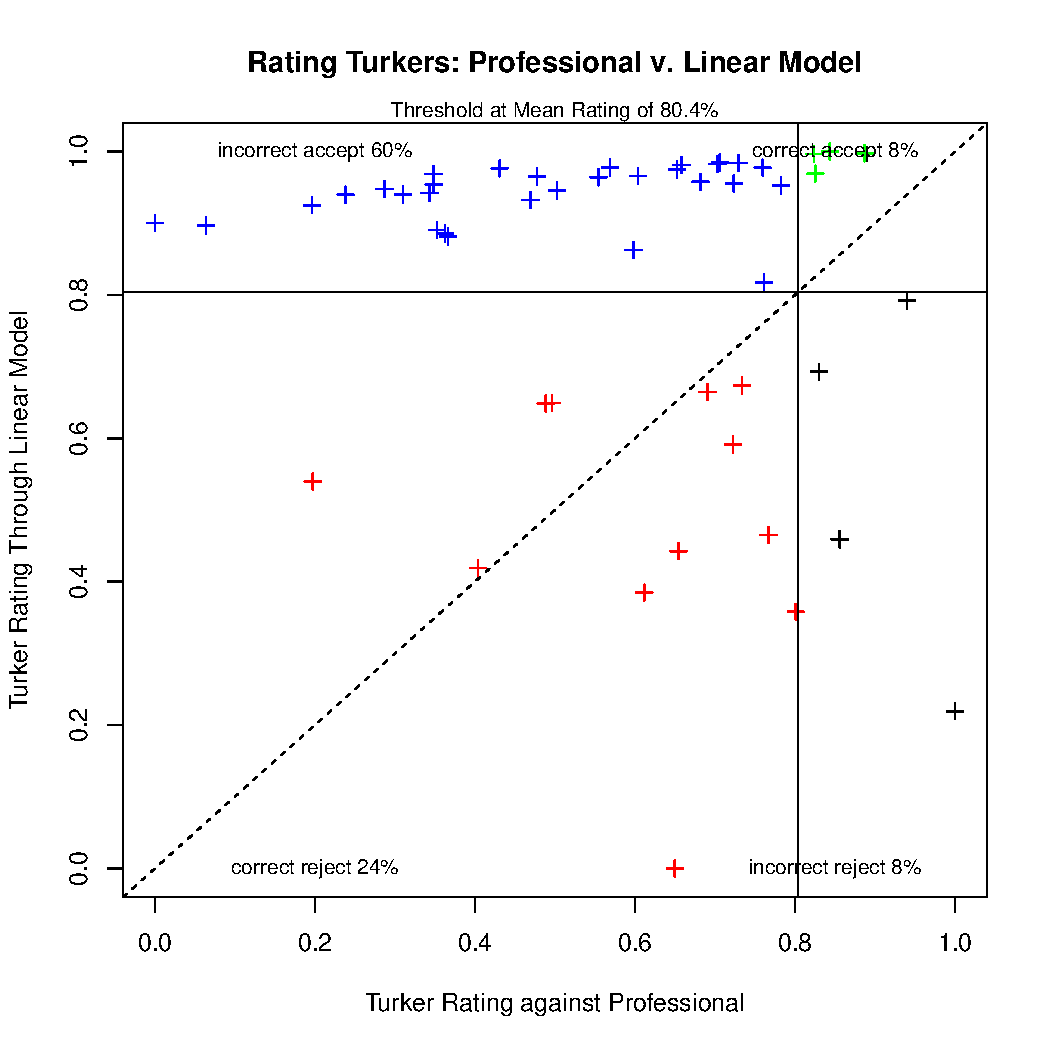
\includegraphics[width=\linewidth]{Senfeature/rrankingsenfeatureranking}
  \caption{Relationship between model predicted rating and gold standard rating. We use sentence level feature to train a linear model. The threshold is the mean of the model predicted rating.}
    \label{flmsenrrating1}
\end{figure}

\begin{figure}[htbp]
  \centering
  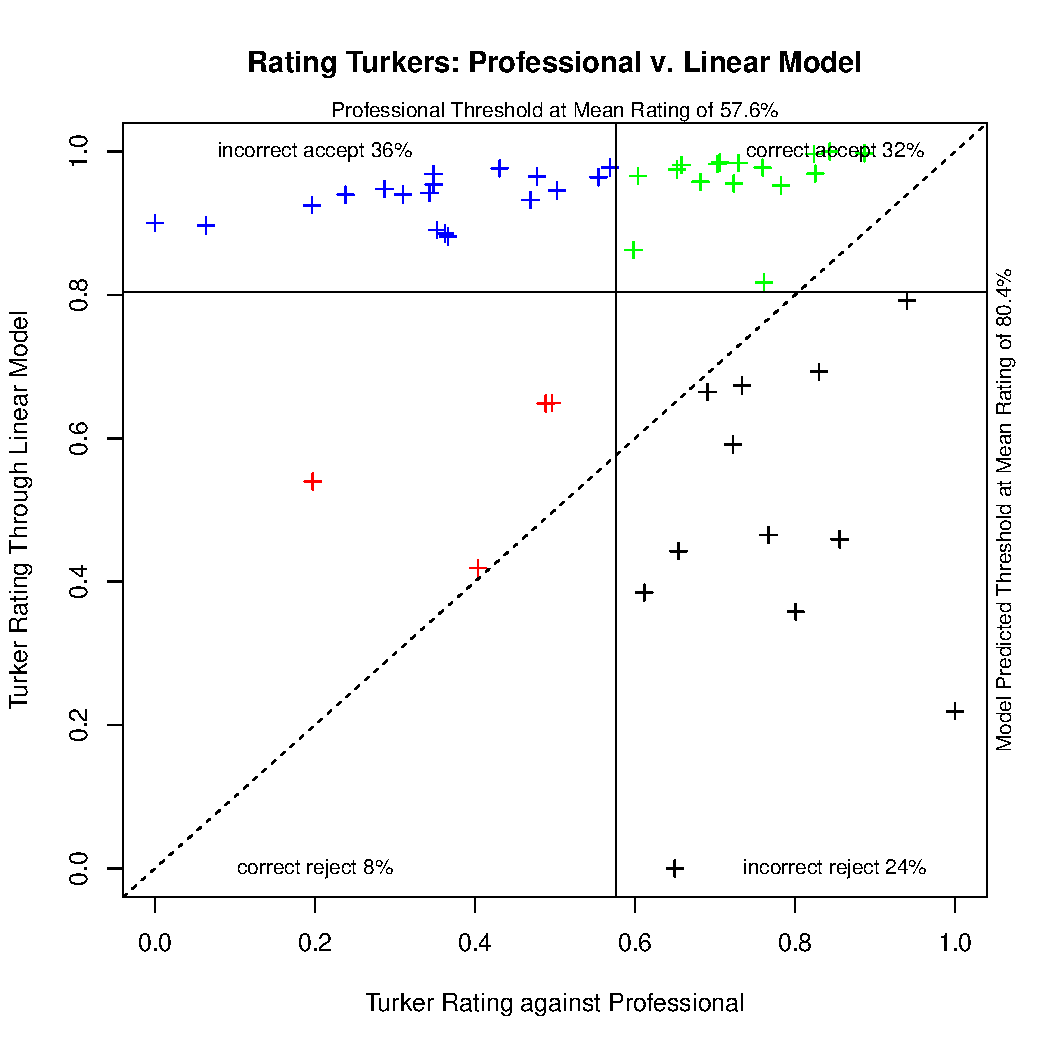
\includegraphics[width=\linewidth]{Senfeature/rrankingsenfeatureranking2}
  \caption{Relationship between model predicted rating and gold standard rating. We use sentence level feature to train a linear model. There are two thresholds: one is the mean of model predicted rating, and the other is the mean of gold standard rating.}
    \label{flmsenrrating2}
\end{figure}

\begin{figure}[htbp]
  \centering
  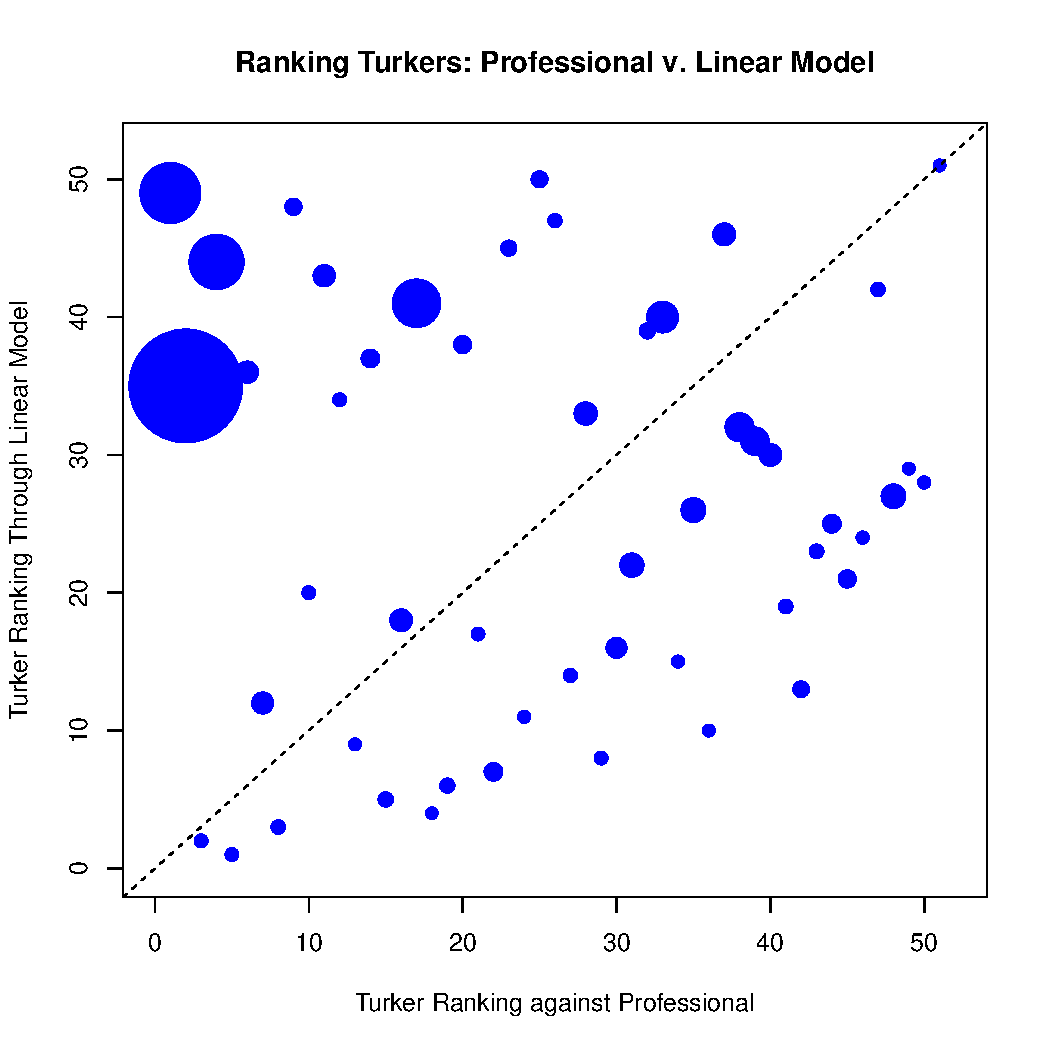
\includegraphics[width=\linewidth]{Senfeature/senrorder}
  \caption{Relationship between gold standard raking and model predicted ranking. We use sentence level feature to train a linear model. }
    \label{flmsenrorder}
\end{figure}
We train the linear model using worker level features to rate workers and rank them. Figure~\ref{flmworkerrrating1} and ~\ref{flmworkerrrating2} show the relation between gold standard rating and model predicted rating. Figure~\ref{flmworkerorder} shows the relation between gold standard ranking and model predicted ranking.
\begin{figure}[htbp]
  \centering
  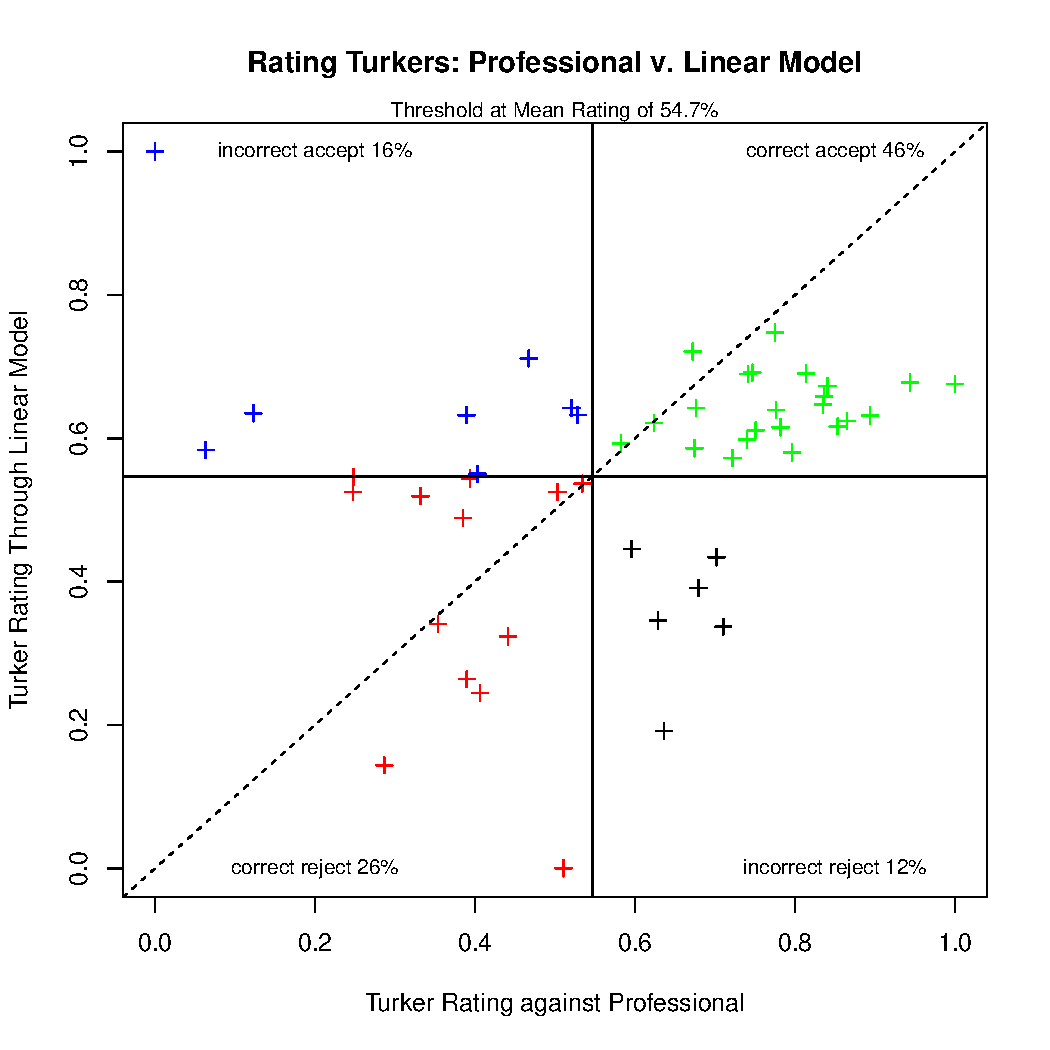
\includegraphics[width=\linewidth]{Workerfeature/rrankingworkerfeaturelm.pdf}
  \caption{Relationship between model predicted rating and gold standard rating. We use worker level feature to train a linear model. The threshold is the mean of the model predicted rating.}
    \label{flmworkerrrating1}
\end{figure}

\begin{figure}[htbp]
  \centering
  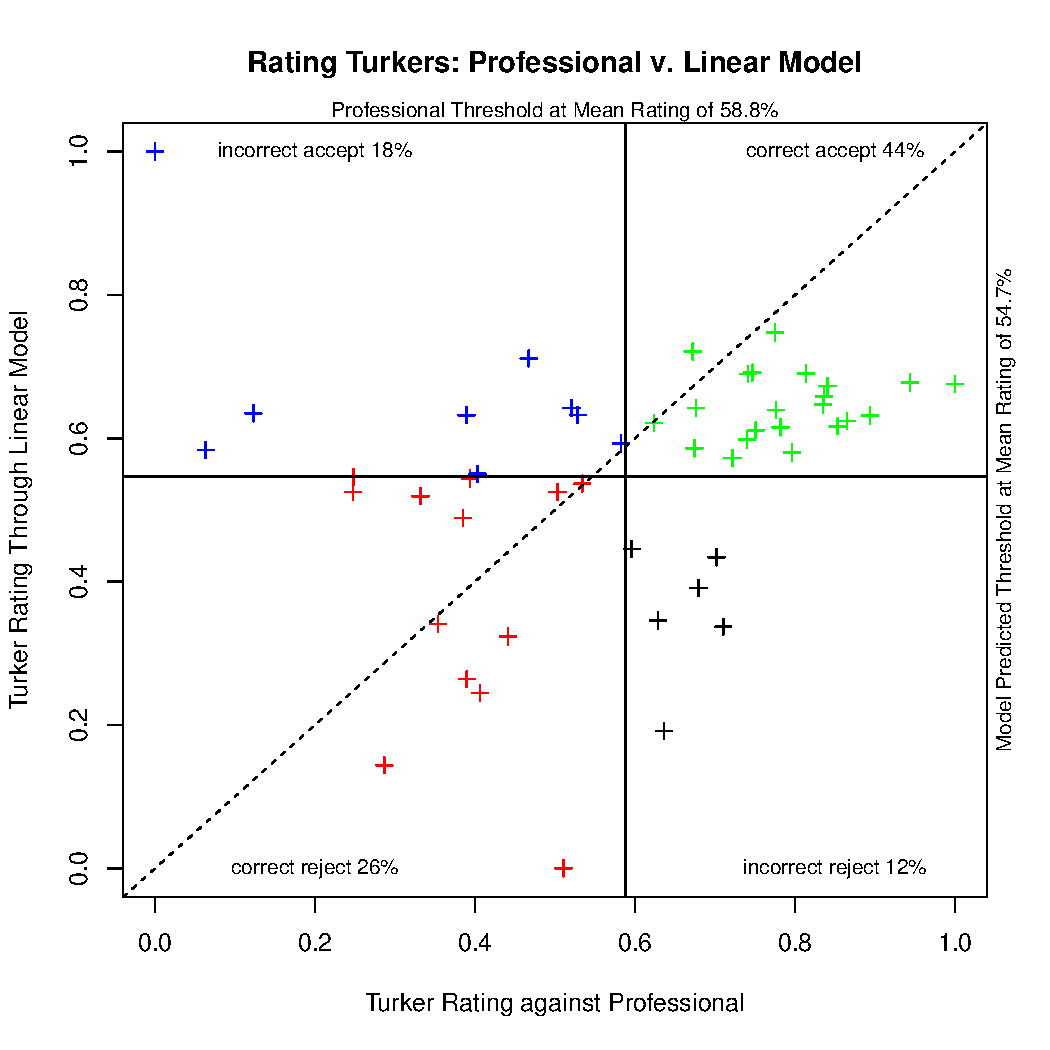
\includegraphics[width=\linewidth]{Workerfeature/rrankingworkerfeaturelm2.pdf}
  \caption{Relationship between model predicted rating and gold standard rating. We use worker level feature to train a linear model. There are two thresholds: one is the mean of model predicted rating, and the other is the mean of gold standard rating.}
    \label{flmworkerrrating2}
\end{figure}

\begin{figure}[htbp]
  \centering
  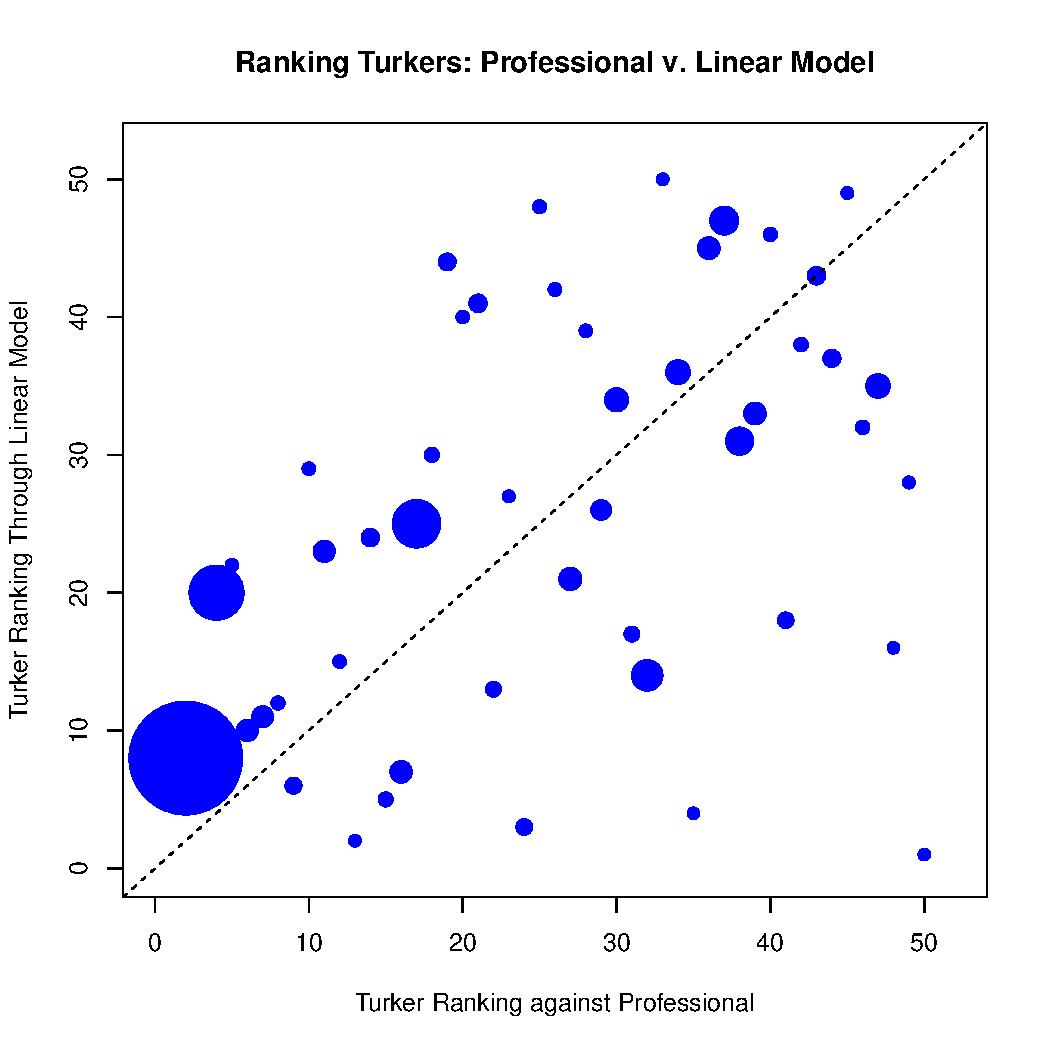
\includegraphics[width=\linewidth]{Workerfeature/workerfeatureorderlm.pdf}
  \caption{Relationship between gold standard ranking and model predicted ranking. We use worker level feature to train a linear model. }
    \label{flmworkerorder}
\end{figure}
We train the linear model using ranking features to rate workers and rank them. Figure~\ref{flmrankingrrating1} and ~\ref{flmrankingrrating2} show the relation between gold standard rating and model predicted rating. Figure~\ref{flmrankingorder} shows the relation between gold standard ranking and model predicted ranking.

\begin{figure}[htbp]
  \centering
  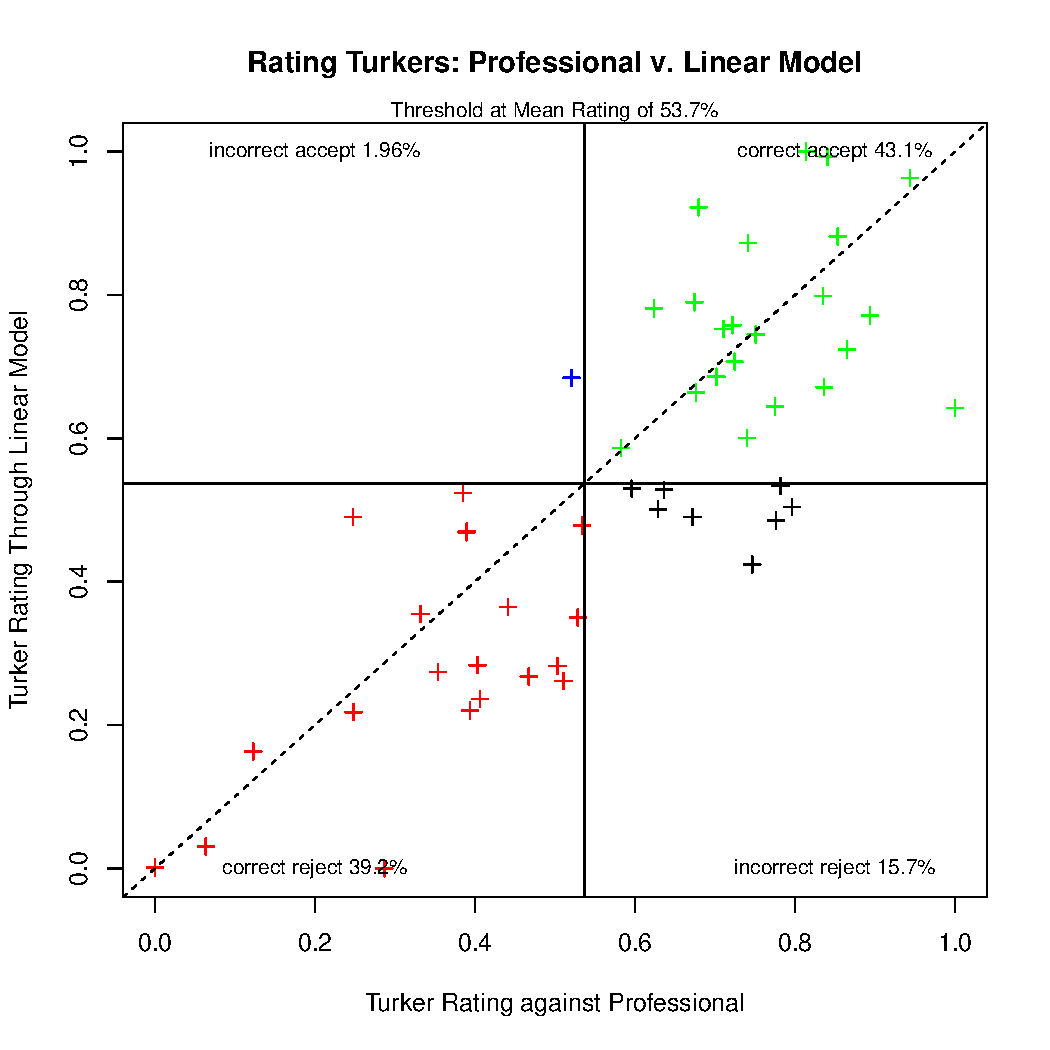
\includegraphics[width=\linewidth]{RankingFeature/rrankingrankingfeaturelm.pdf}
  \caption{Relationship between model predicted rating and gold standard rating. We use ranking feature to train a linear model. The threshold is the mean of the model predicted rating.}
    \label{flmrankingrrating1}
\end{figure}

\begin{figure}[htbp]
  \centering
  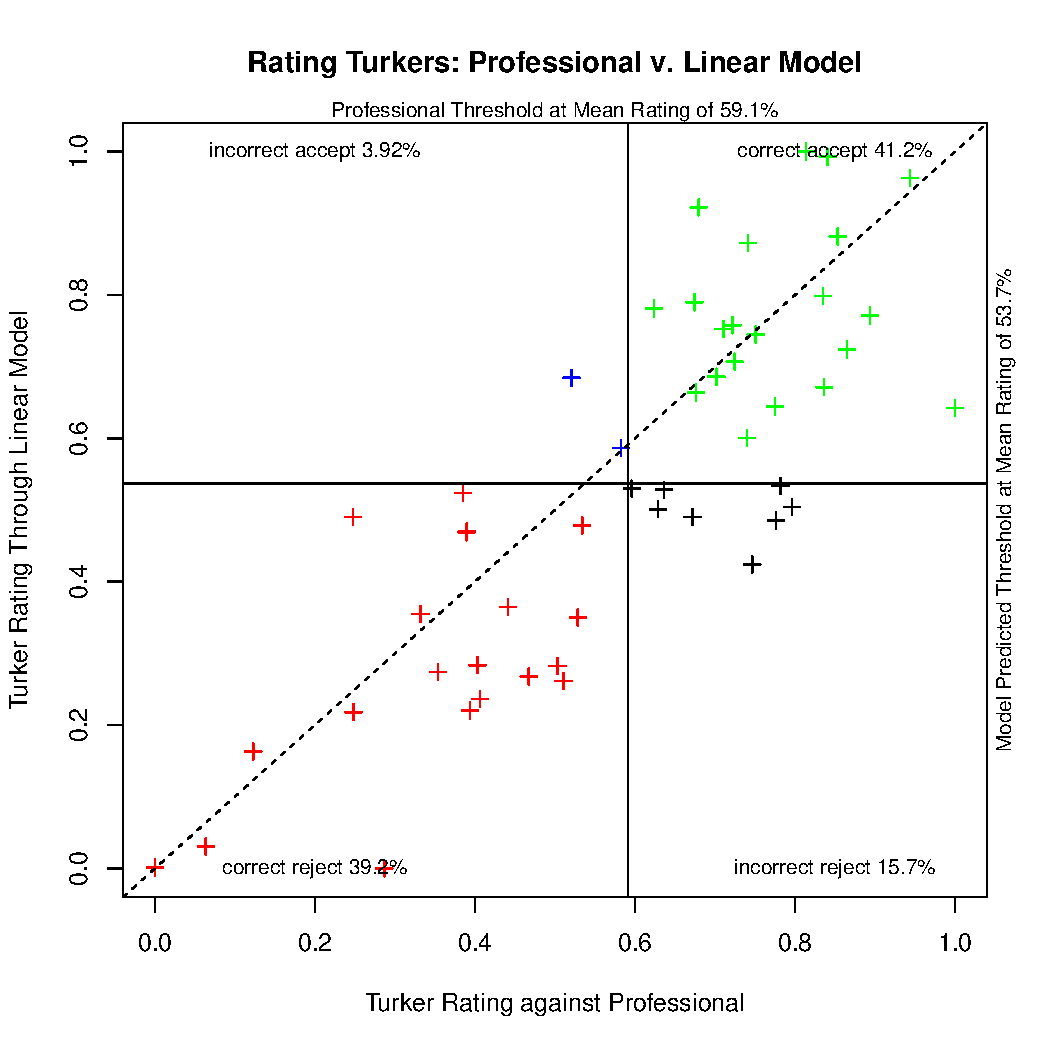
\includegraphics[width=\linewidth]{RankingFeature/rrankingrankingfeaturelm2.pdf}
  \caption{Relationship between model predicted rating and gold standard rating. We use ranking feature to train a linear model. There are two thresholds: one is the mean of model predicted rating, and the other is the mean of gold standard rating.}
    \label{flmrankingrrating2}
\end{figure}

\begin{figure}[htbp]
  \centering
  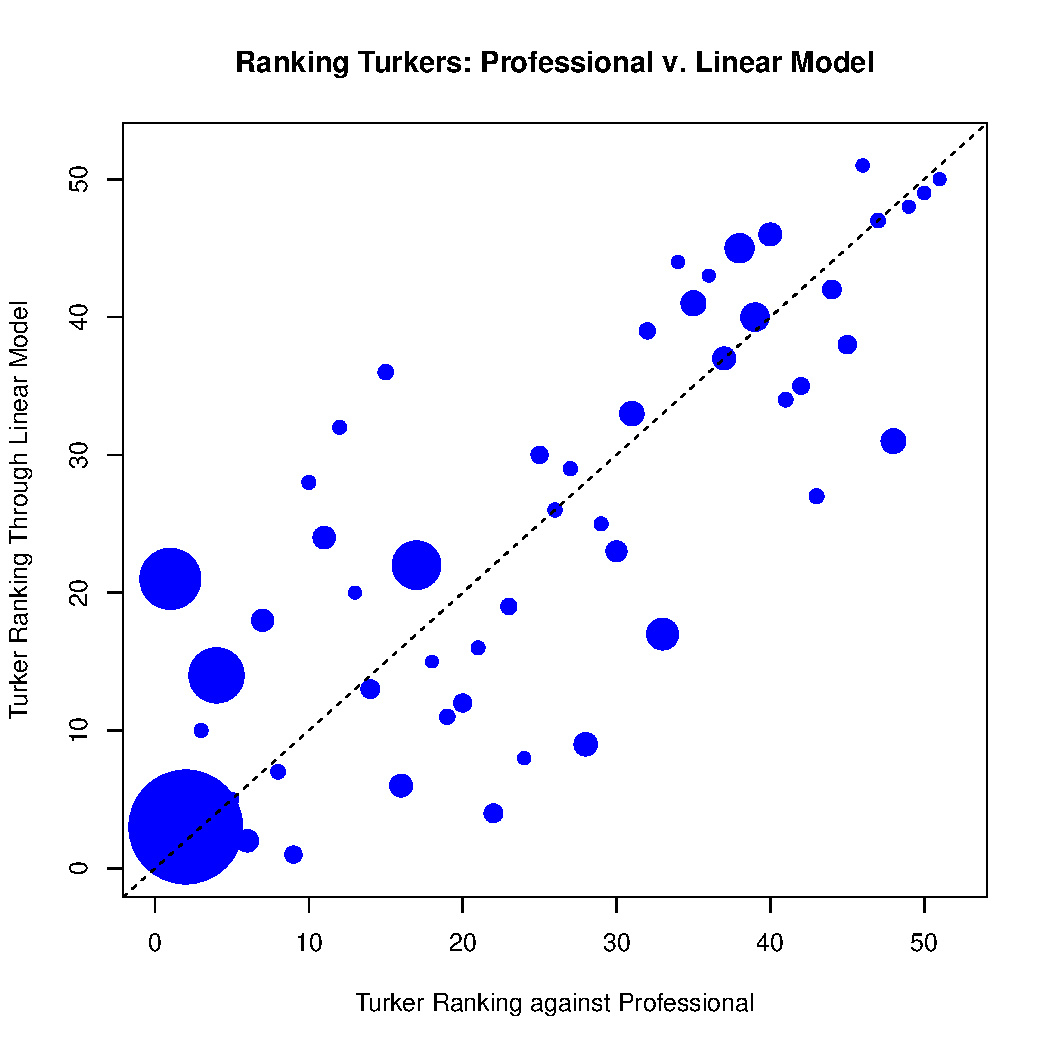
\includegraphics[width=\linewidth]{RankingFeature/rankfeatureorderlm.pdf}
  \caption{Relationship between gold standard ranking and model predicted ranking. We use ranking feature to train a linear model. }
    \label{flmrankingorder}
\end{figure}
We train the linear model using all features with calibration to rate workers and rank them. Figure~\ref{flmallcalirrating1} and ~\ref{flmallcalirrating2} show the relation between gold standard rating and model predicted rating. Figure~\ref{flmallcaliorder} shows the relation between gold standard ranking and model predicted ranking.

\begin{figure}[htbp]
  \centering
  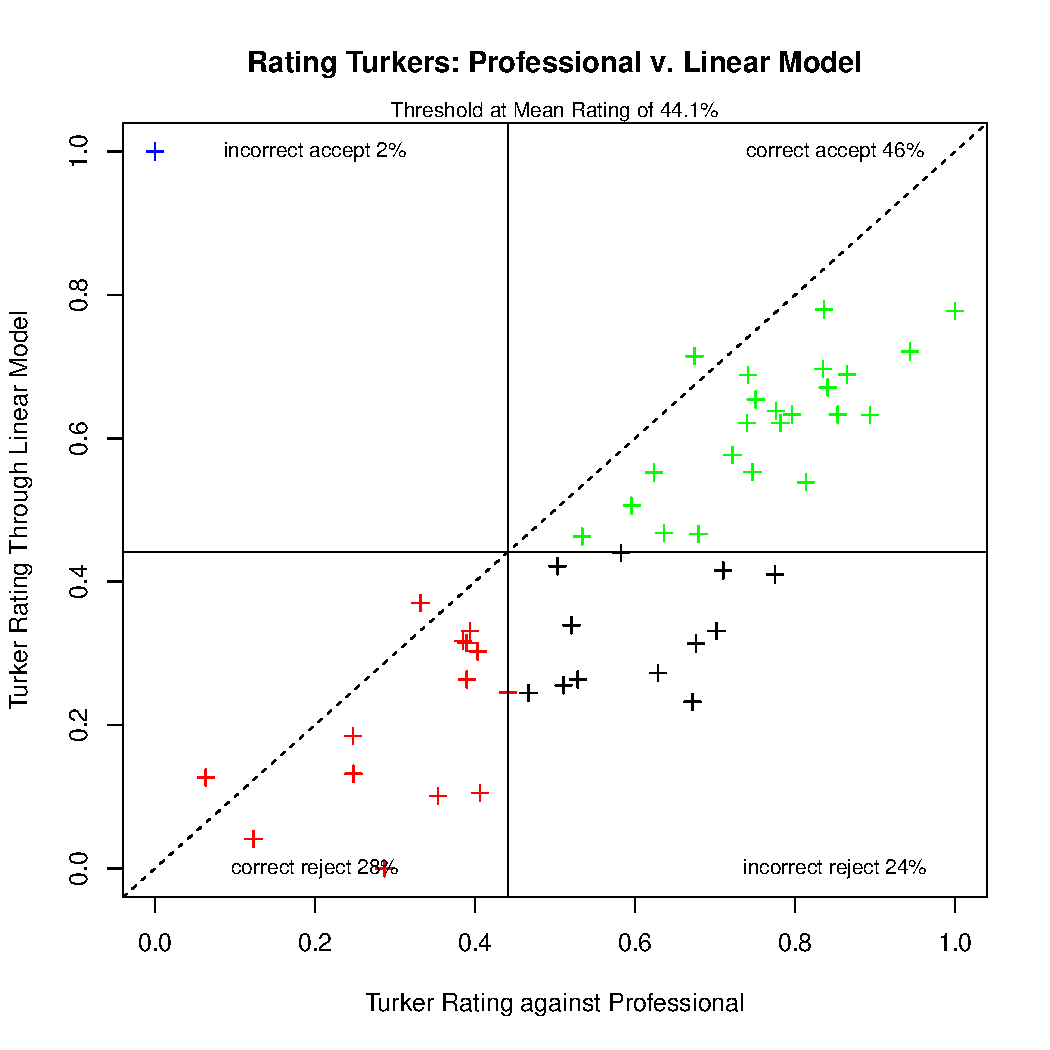
\includegraphics[width=\linewidth]{AllFeatureWithCali/rrankingallfeaturewithcalilm.pdf}
  \caption{Relationship between model predicted rating and gold standard rating. We use all features (calibration) to train a linear model. The threshold is the mean of the model predicted rating.}
    \label{flmallcalirrating1}
\end{figure}

\begin{figure}[htbp]
  \centering
  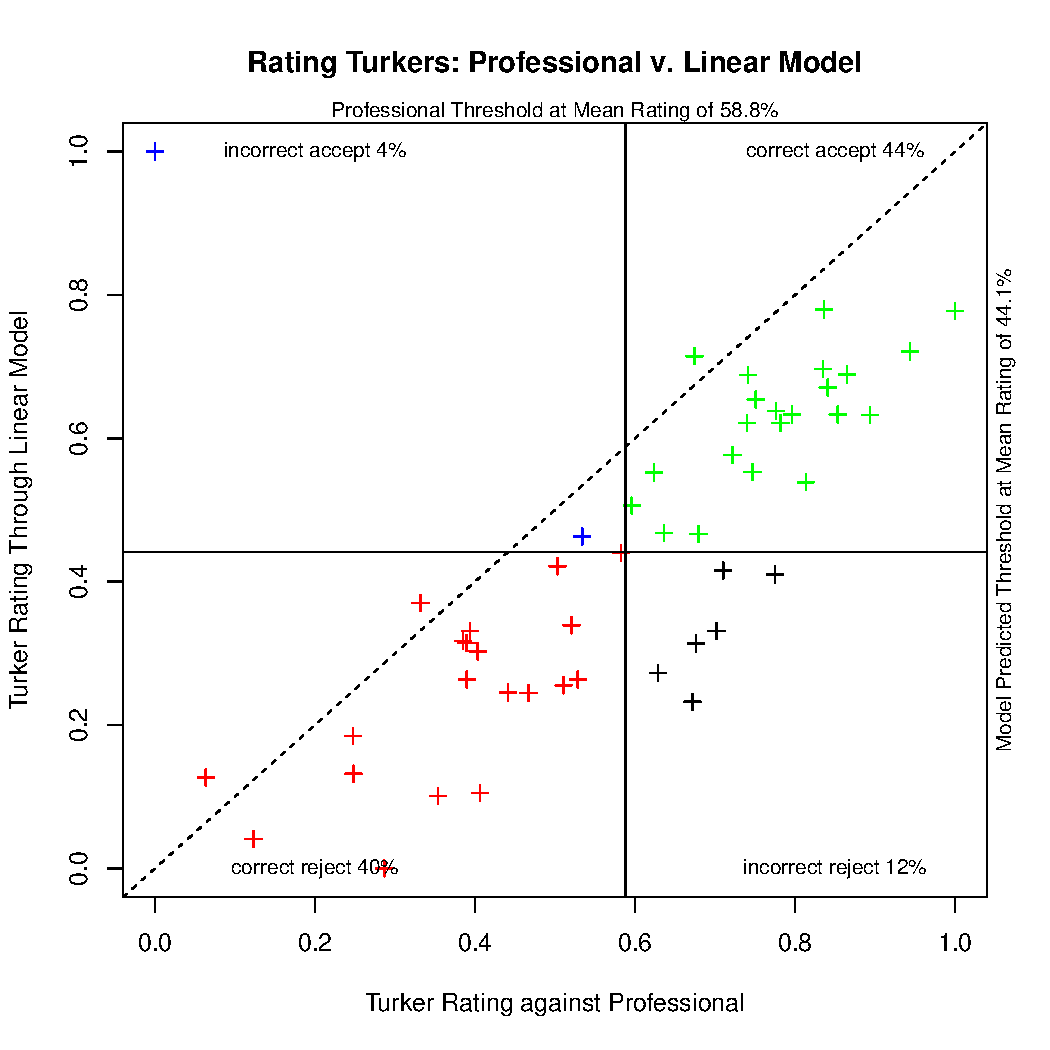
\includegraphics[width=\linewidth]{AllFeatureWithCali/rrankingallfeaturewithcalilm2.pdf}
  \caption{Relationship between model predicted rating and gold standard rating. We use all features (calibration) to train a linear model. There are two thresholds: one is the mean of model predicted rating, and the other is the mean of gold standard rating.}
    \label{flmallcalirrating2}
\end{figure}

\begin{figure}[htbp]
  \centering
  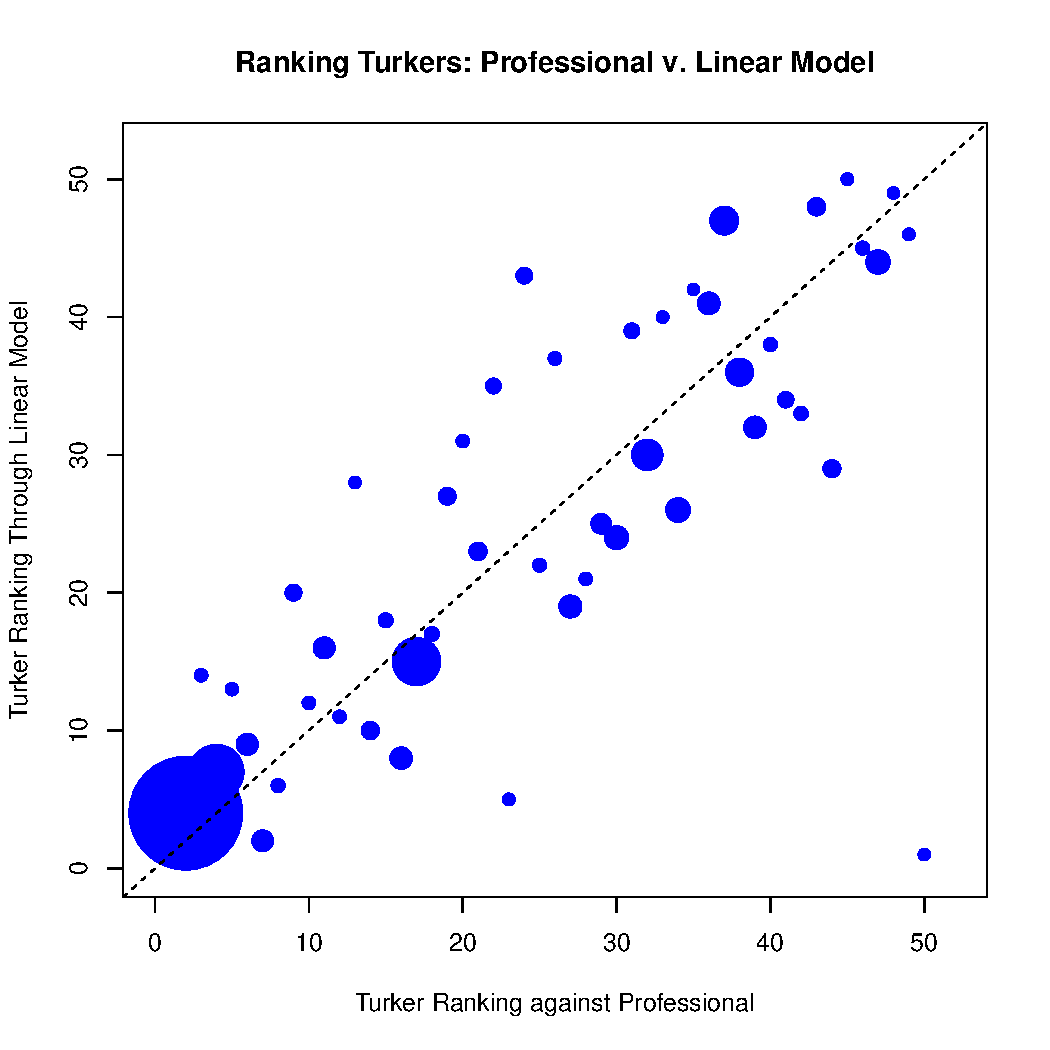
\includegraphics[width=\linewidth]{AllFeatureWithCali/allfeaturewithcaliorderlm.pdf}
  \caption{Relationship between gold standard ranking and model predicted ranking. We use all features (calibration) to train a linear model. }
    \label{flmallcaliorder}
\end{figure}

\subsubsection{Decision Tree Model}
We also implement a decision tree model to rank workers.
\begin{table}[htbp]
\begin{center}
\begin{tabular}{| l | c | r |}
\hline \bf Feature Set & \bf Prson's  &\bf Sprman's  \\ \hline
Sentence features & 0.86& 0.86 \\
Worker level feature & 0.88  & 0.88 \\
Ranking feature & 0.84 & 0.84 \\
Calibration feature & 0.98& 0.98\\
All features (Calibration)& 0.95 & 0.95 \\
\hline
\end{tabular}
\end{center}
\caption{\label{tdtpearson} Pearson's Correlation for Decision Tree Model trained from different feature set }
\end{table}
We train the decision tree model using sentence level features to rate workers and rank them. Figure~\ref{fdtsenrrating1} and ~\ref{fdtsenrrating2} show the relation between gold standard rating and model predicted rating. Figure~\ref{fdtsenrorder} shows the relation between gold standard ranking and model predicted ranking.

\begin{figure}[htbp]
  \centering
  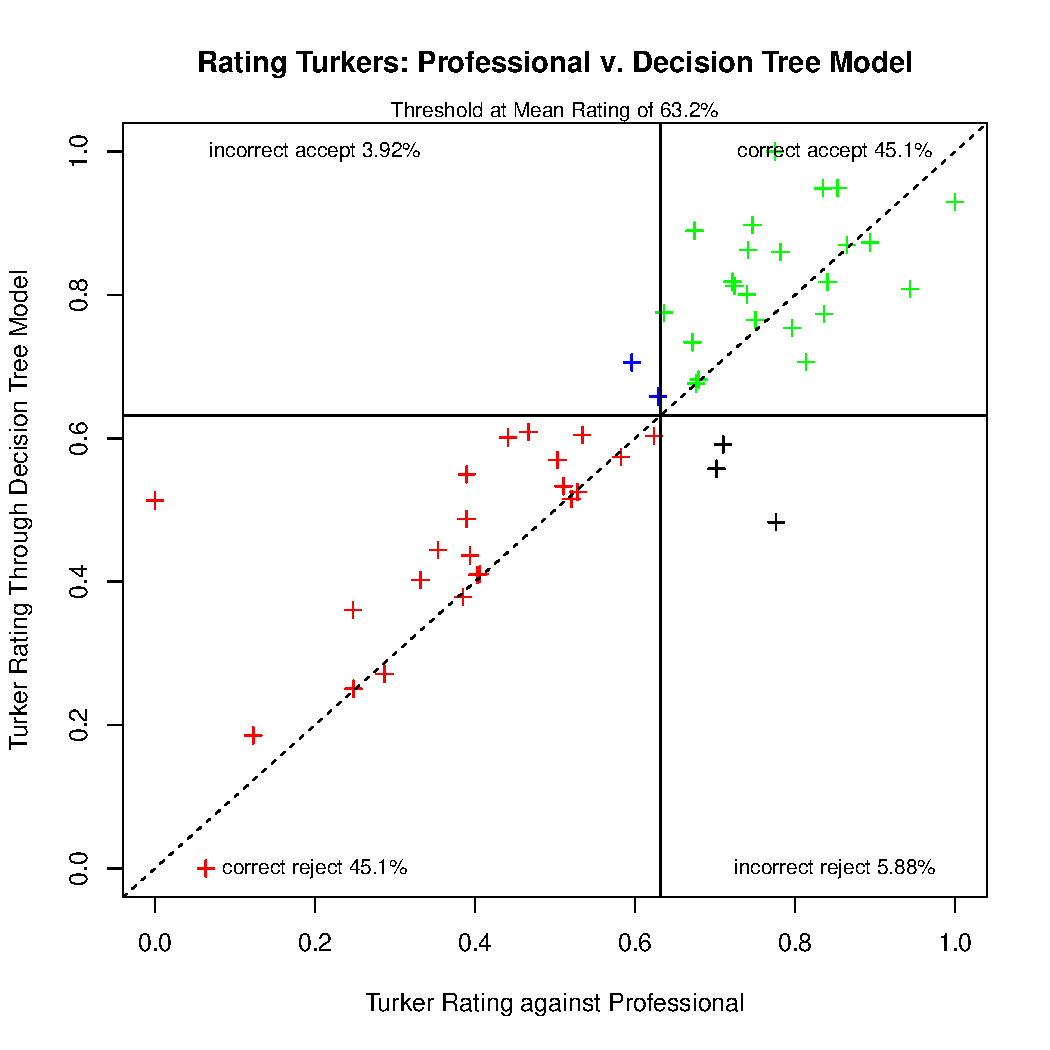
\includegraphics[width=\linewidth]{Senfeature/rrankingsenfeatureDT}
  \caption{Relationship between model predicted rating and gold standard rating. We use sentence level feature to train a Decision Tree model. The threshold is the mean of the model predicted rating.}
    \label{fdtsenrrating1}
\end{figure}

\begin{figure}[htbp]
  \centering
  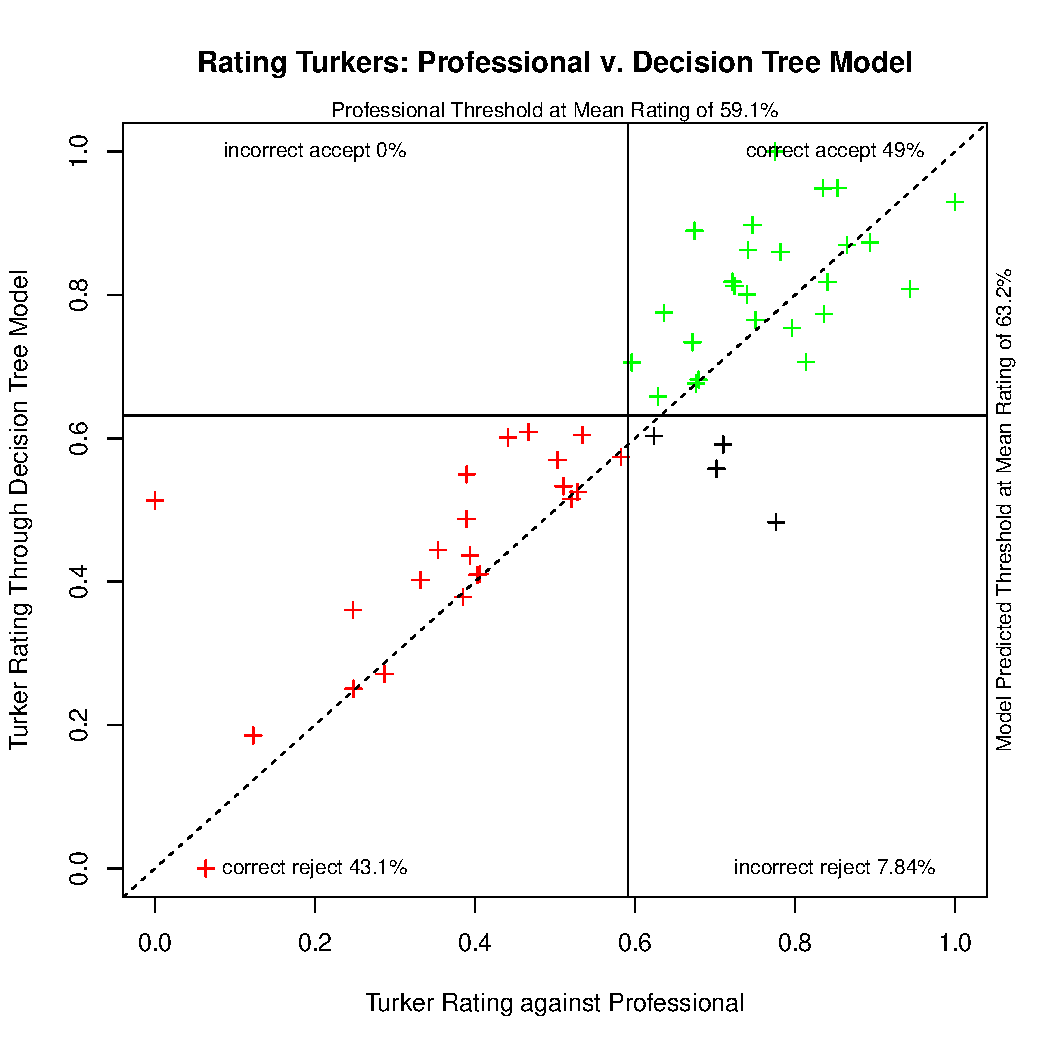
\includegraphics[width=\linewidth]{Senfeature/rrankingsenfeatureDT2}
  \caption{Relationship between model predicted rating and gold standard rating. We use sentence level feature to train a Decision Tree model. There are two thresholds: one is the mean of model predicted rating, and the other is the mean of gold standard rating.}
    \label{fdtsenrrating2}
\end{figure}

\begin{figure}[htbp]
  \centering
  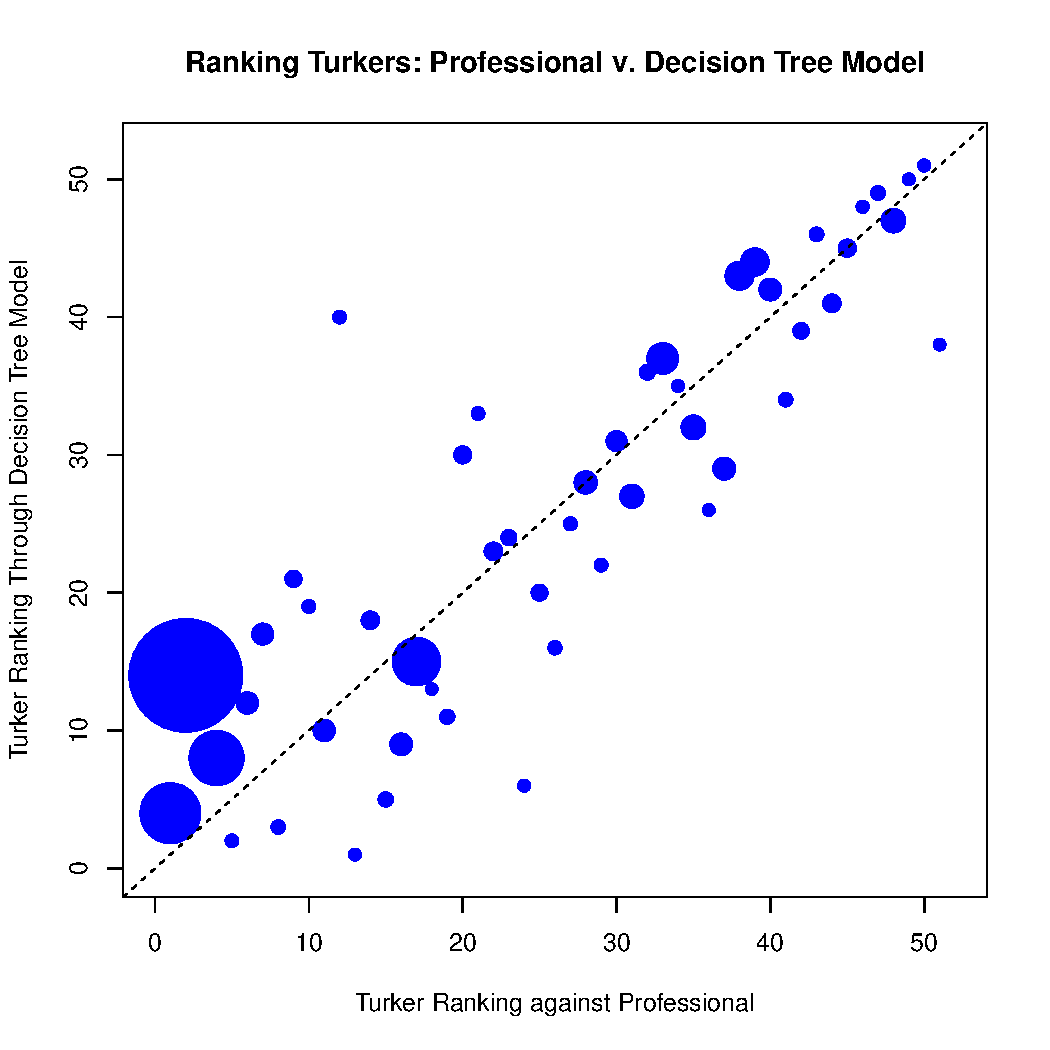
\includegraphics[width=\linewidth]{Senfeature/senroederDT}
  \caption{Relationship between gold standard raking and model predicted ranking. We use sentence level feature to train a Decision Tree model. }
    \label{fdtsenrorder}
\end{figure}
We train the decision tree model using worker level features to rate workers and rank them. Figure~\ref{fdtworkerrrating1} and ~\ref{fdtworkerrrating2} show the relation between gold standard rating and model predicted rating. Figure~\ref{fdtworkerorder} shows the relation between gold standard ranking and model predicted ranking.

\begin{figure}[htbp]
  \centering
  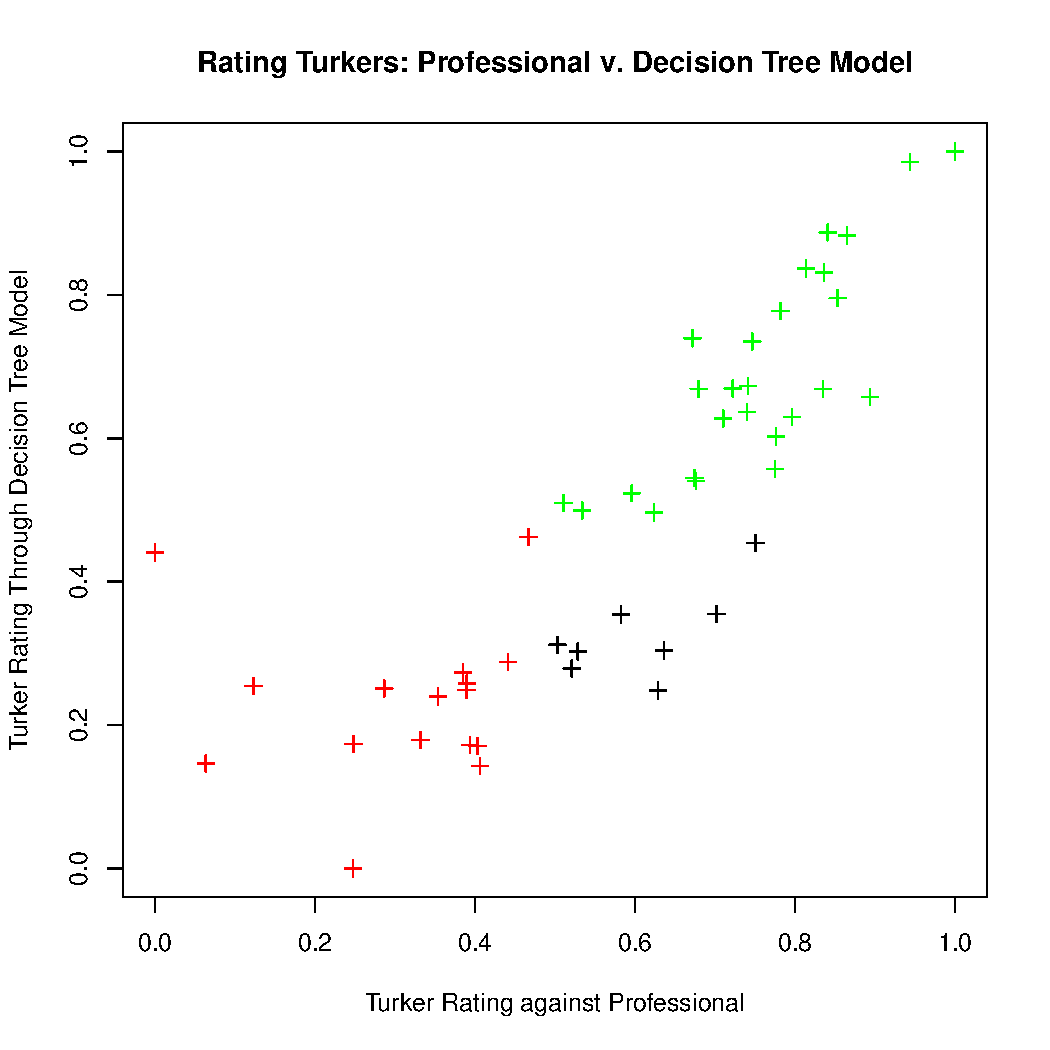
\includegraphics[width=\linewidth]{Workerfeature/rrankingworkerfeaturedt.pdf}
  \caption{Relationship between model predicted rating and gold standard rating. We use worker level feature to train a Decision Tree model. The threshold is the mean of the model predicted rating.}
    \label{fdtworkerrrating1}
\end{figure}

\begin{figure}[htbp]
  \centering
  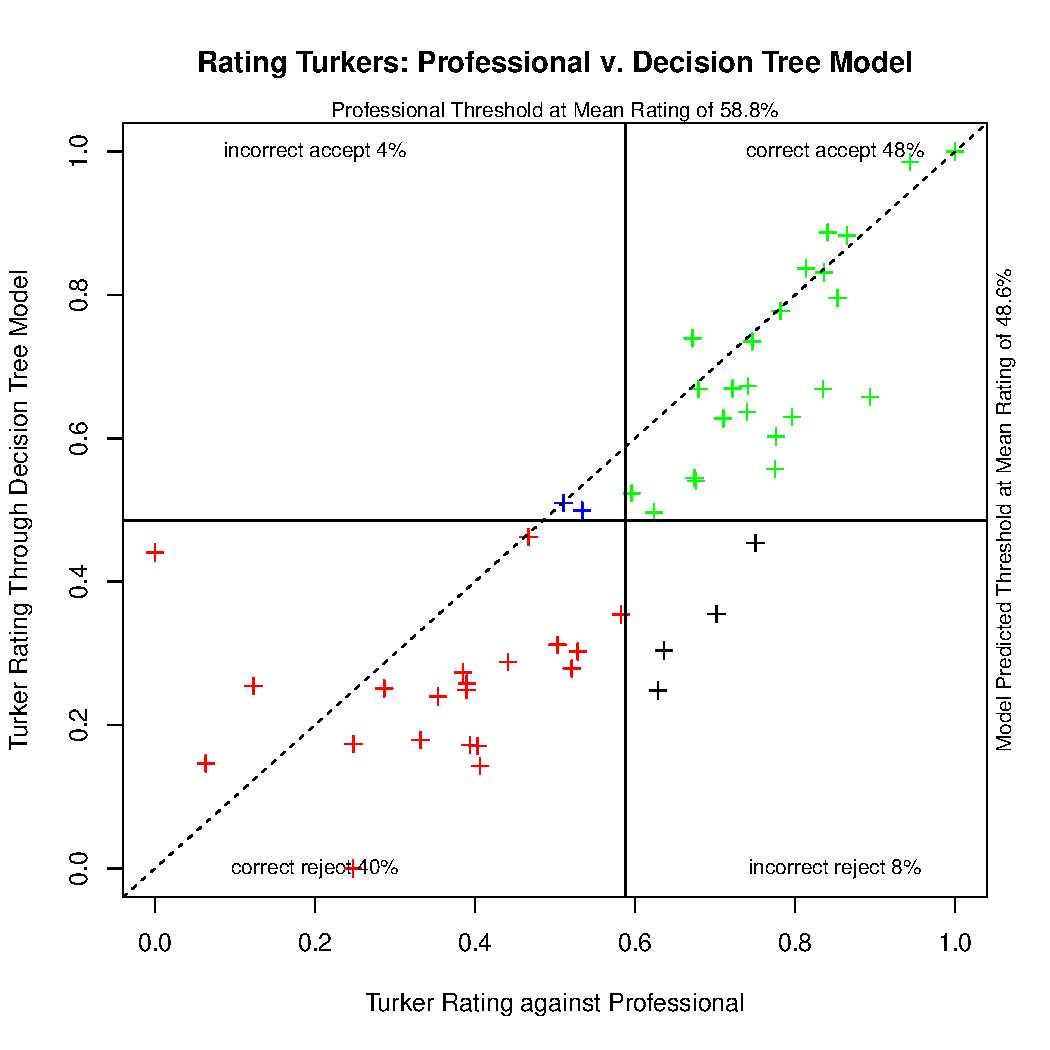
\includegraphics[width=\linewidth]{Workerfeature/rrankingworkerfeaturedt2.pdf}
  \caption{Relationship between model predicted rating and gold standard rating. We use worker level feature to train a Decision Tree model. There are two thresholds: one is the mean of model predicted rating, and the other is the mean of gold standard rating.}
    \label{fdtworkerrrating2}
\end{figure}

\begin{figure}[htbp]
  \centering
  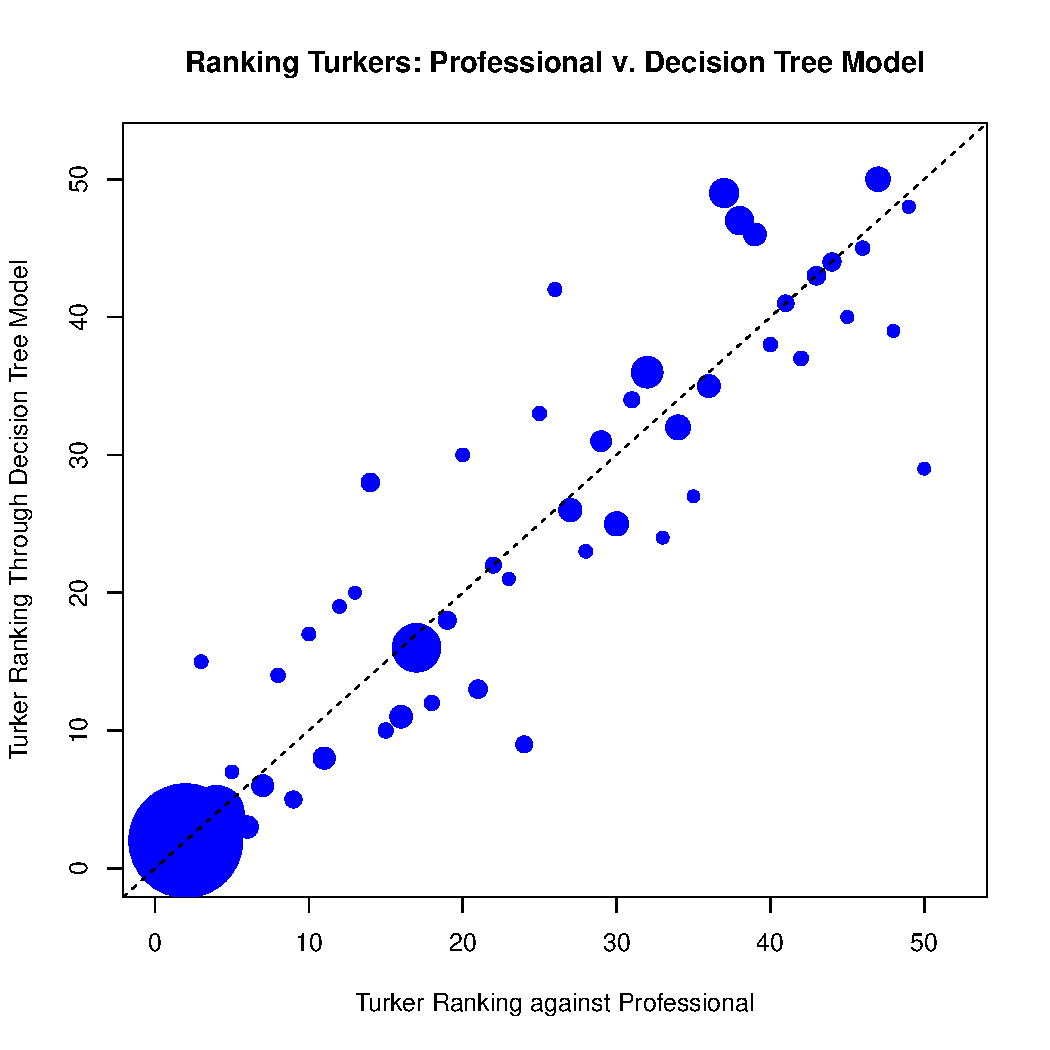
\includegraphics[width=\linewidth]{Workerfeature/workerfeatureorderdt.pdf}
  \caption{Relationship between gold standard raking and model predicted ranking. We use worker level feature to train a Decision Tree model. }
    \label{fdtworkerorder}
\end{figure}

We train the decision tree model using ranking features to rate workers and rank them. Figure~\ref{fdtrankingrrating1} and ~\ref{fdtrankingrrating2} show the relation between gold standard rating and model predicted rating. Figure~\ref{fdtrankingrorder} shows the relation between gold standard ranking and model predicted ranking.

\begin{figure}[htbp]
  \centering
  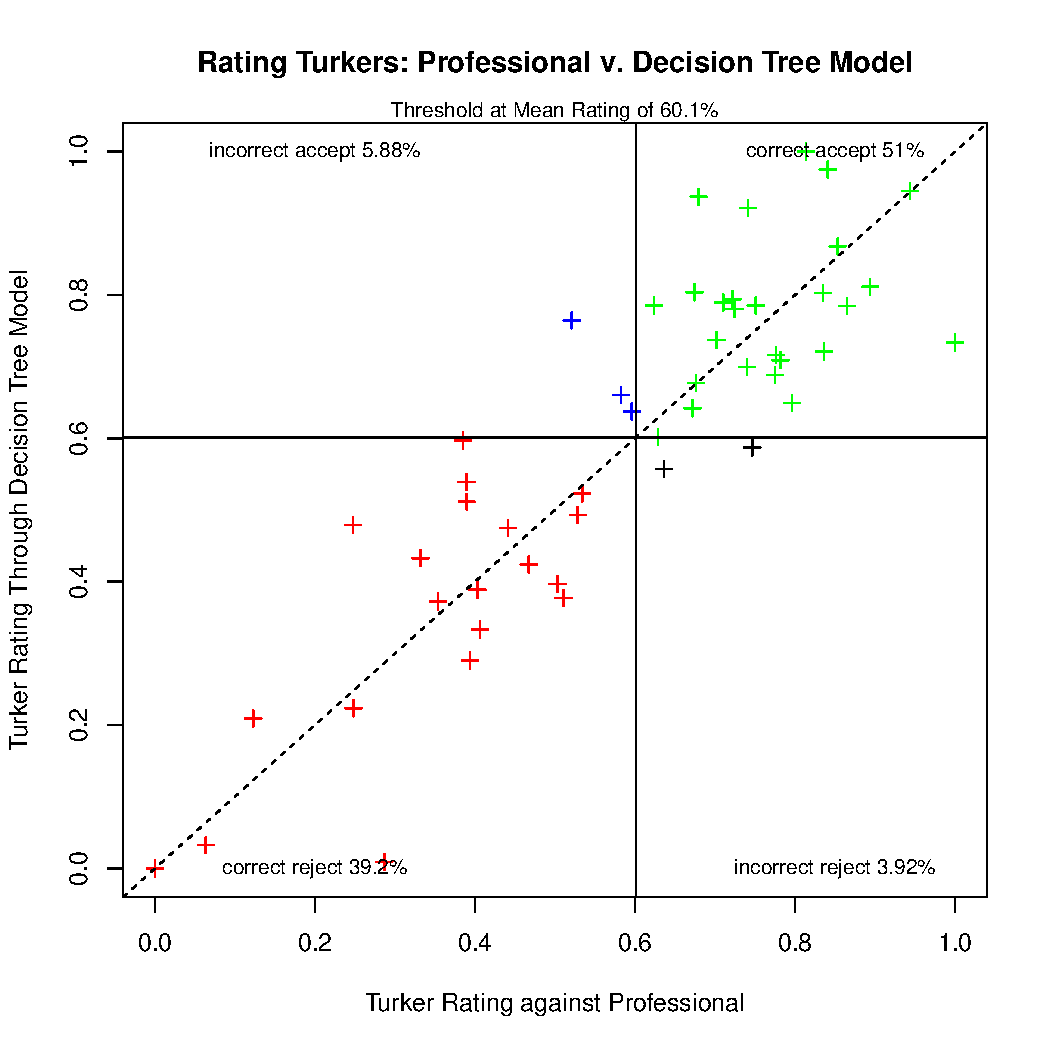
\includegraphics[width=\linewidth]{Rankingfeature/rrankingrankingfeaturedt.pdf}
  \caption{Relationship between model predicted rating and gold standard rating. We use ranking level feature to train a Decision Tree model. The threshold is the mean of the model predicted rating.}
    \label{fdtrankingrrating1}
\end{figure}

\begin{figure}[htbp]
  \centering
  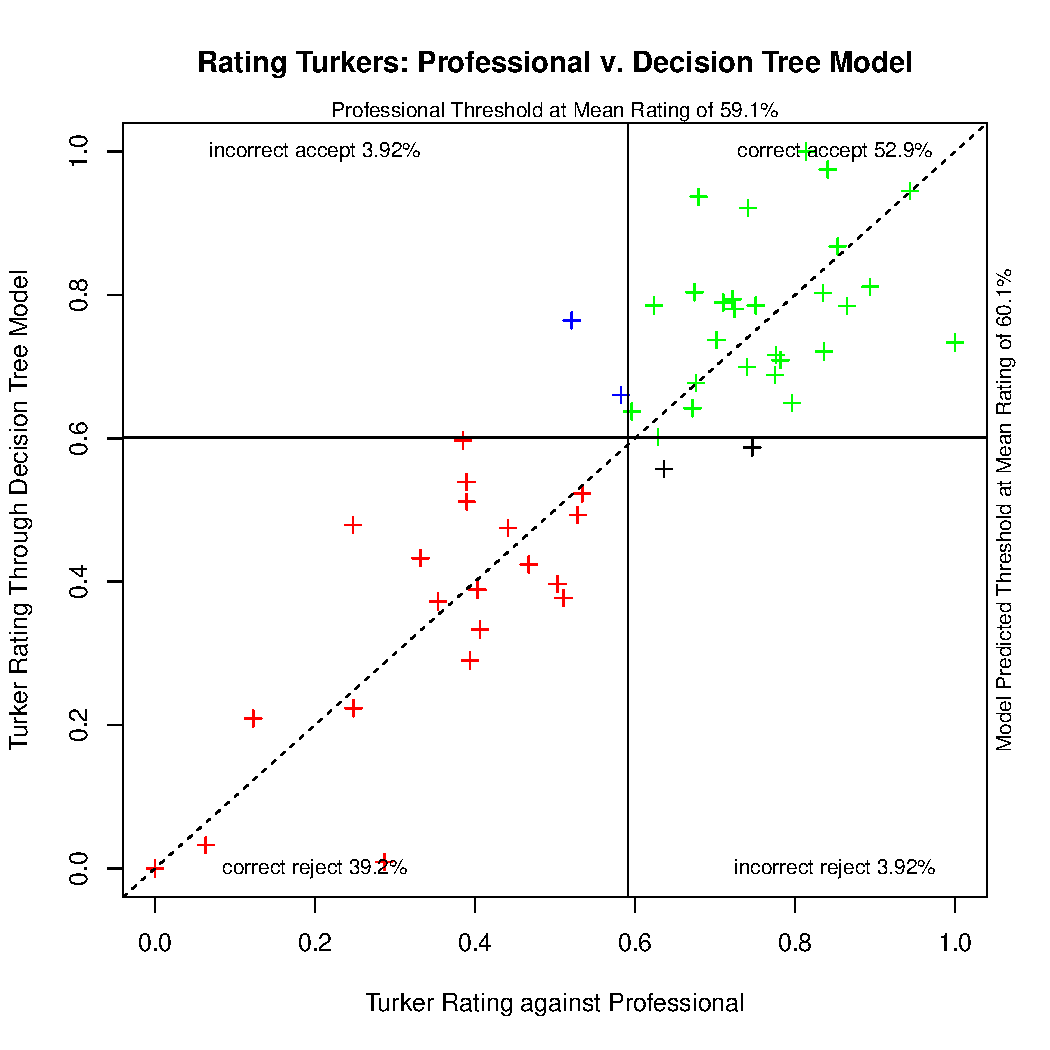
\includegraphics[width=\linewidth]{Rankingfeature/rrankingrankingfeaturedt2.pdf}
  \caption{Relationship between model predicted rating and gold standard rating. We use ranking  feature to train a Decision Tree model. There are two thresholds: one is the mean of model predicted rating, and the other is the mean of gold standard rating.}
    \label{fdtrankingrrating2}
\end{figure}

\begin{figure}[htbp]
  \centering
  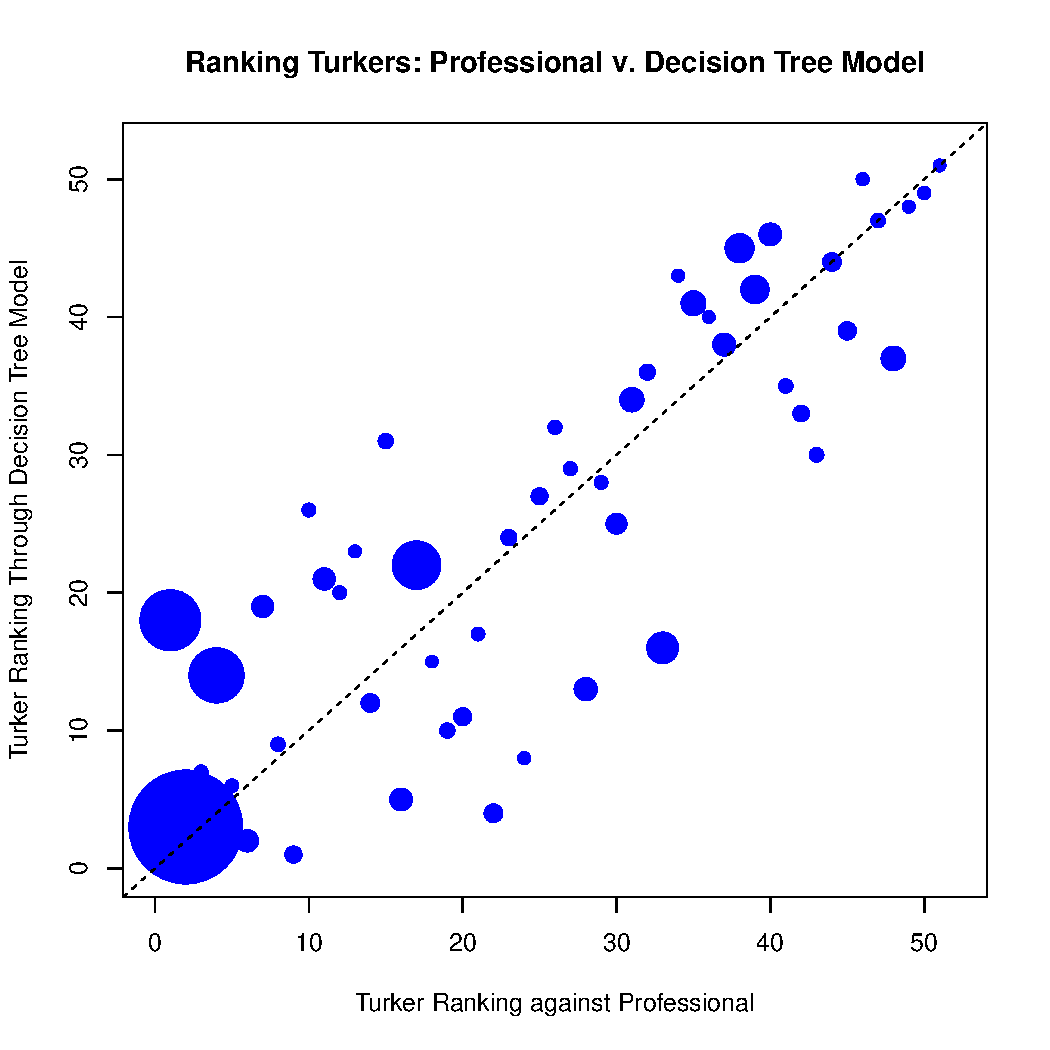
\includegraphics[width=\linewidth]{Rankingfeature/rankfeatureorderdt.pdf}
  \caption{Relationship between gold standard raking and model predicted ranking. We use ranking level feature to train a Decision Tree model. }
    \label{fdtrankingrorder}
\end{figure}

We train the decision tree model using all features with calibration to rate workers and rank them. Figure~\ref{fdtallcalirrating1} and Figure ~\ref{fdtallcalirrating2} show the relation between gold standard rating and model predicted rating. Figure~\ref{fdtallcalirorder} shows the relation between gold standard ranking and model predicted ranking.

\begin{figure}[htbp]
  \centering
  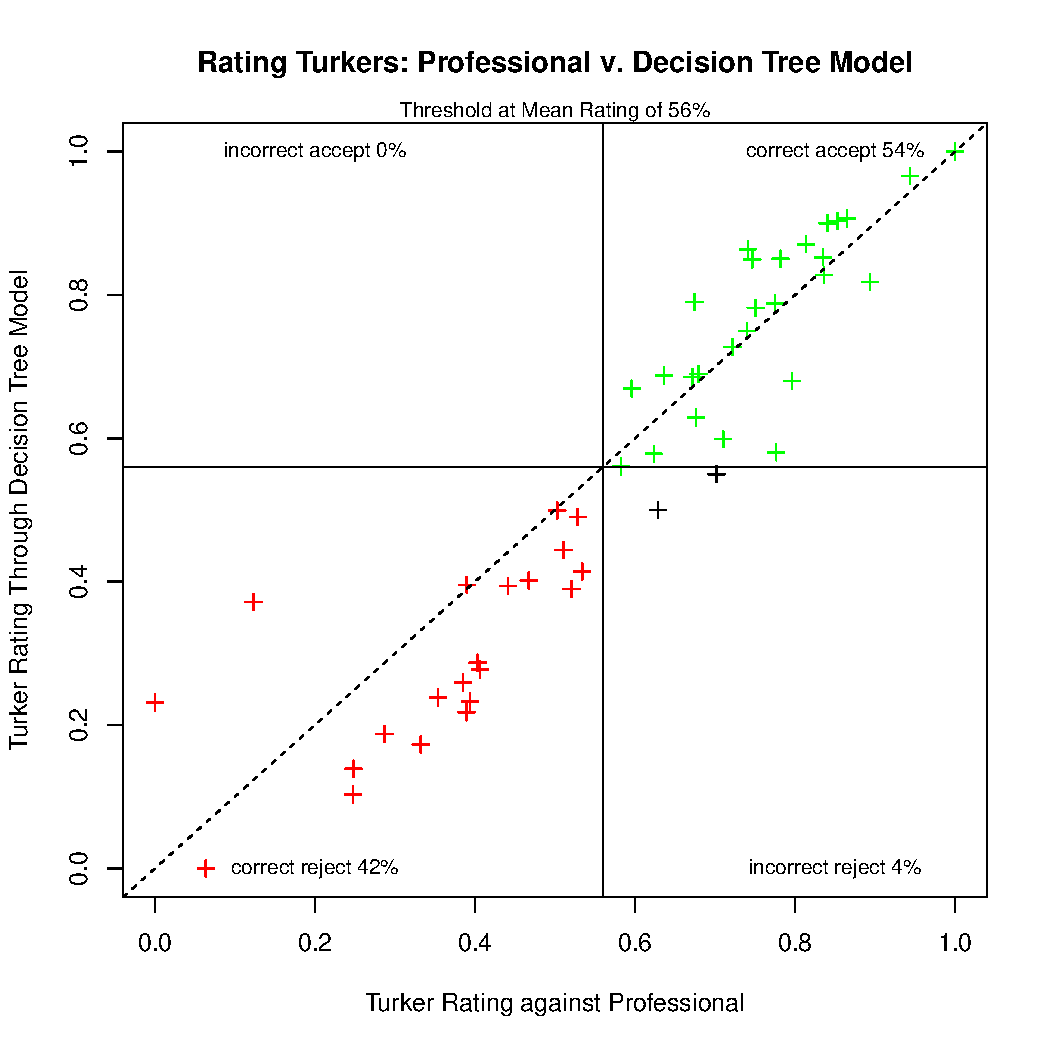
\includegraphics[width=\linewidth]{AllFeatureWithCali/rrankingallfeaturewithcalidt.pdf}
  \caption{Relationship between model predicted rating and gold standard rating. We use all features with calibration to train a Decision Tree model. The threshold is the mean of the model predicted rating.}
    \label{fdtallcalirrating1}
\end{figure}

\begin{figure}[htbp]
  \centering
  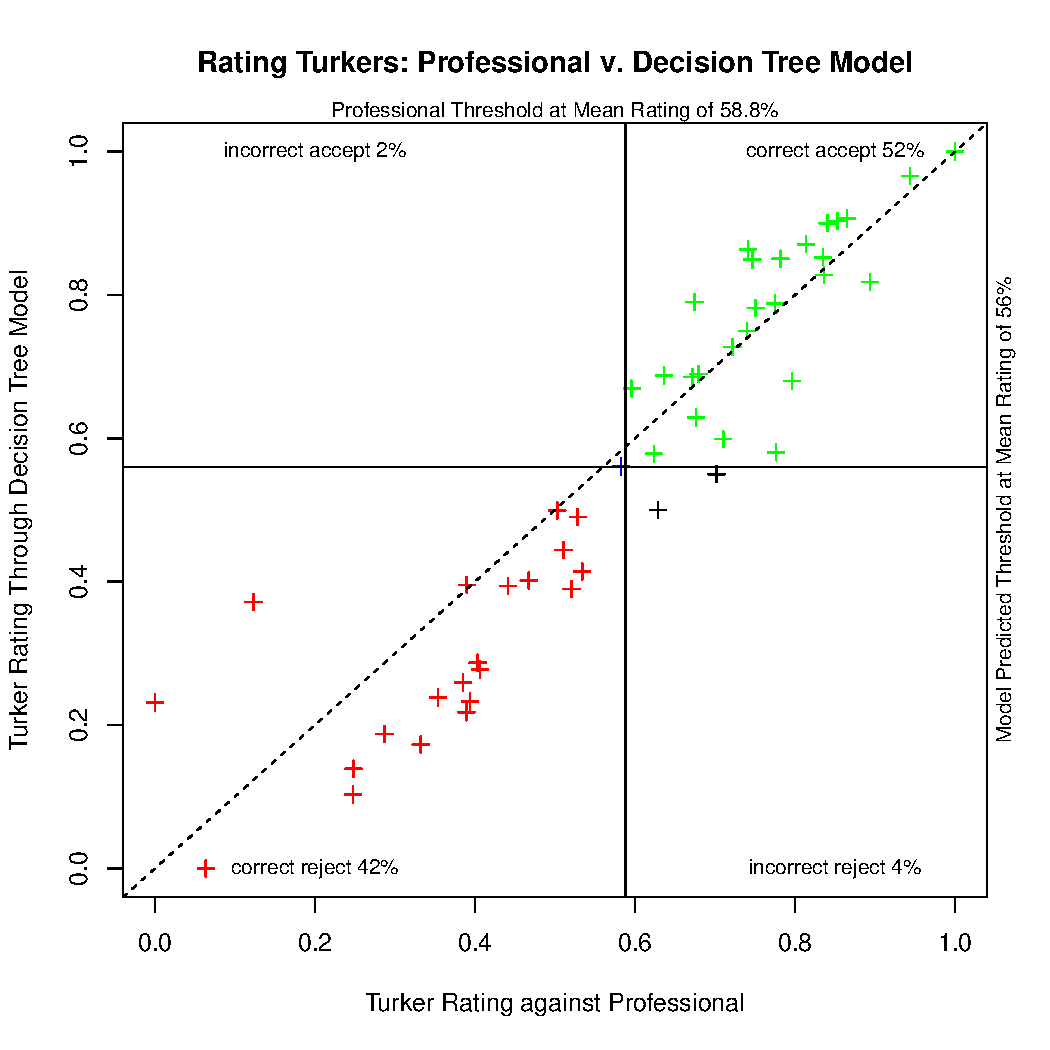
\includegraphics[width=\linewidth]{AllFeatureWithCali/rrankingallfeaturewithcalidt2.pdf}
  \caption{Relationship between model predicted rating and gold standard rating. We use all features with calibration to train a Decision Tree model. There are two thresholds: one is the mean of model predicted rating, and the other is the mean of gold standard rating.}
    \label{fdtallcalirrating2}
\end{figure}

\begin{figure}[htbp]
  \centering
  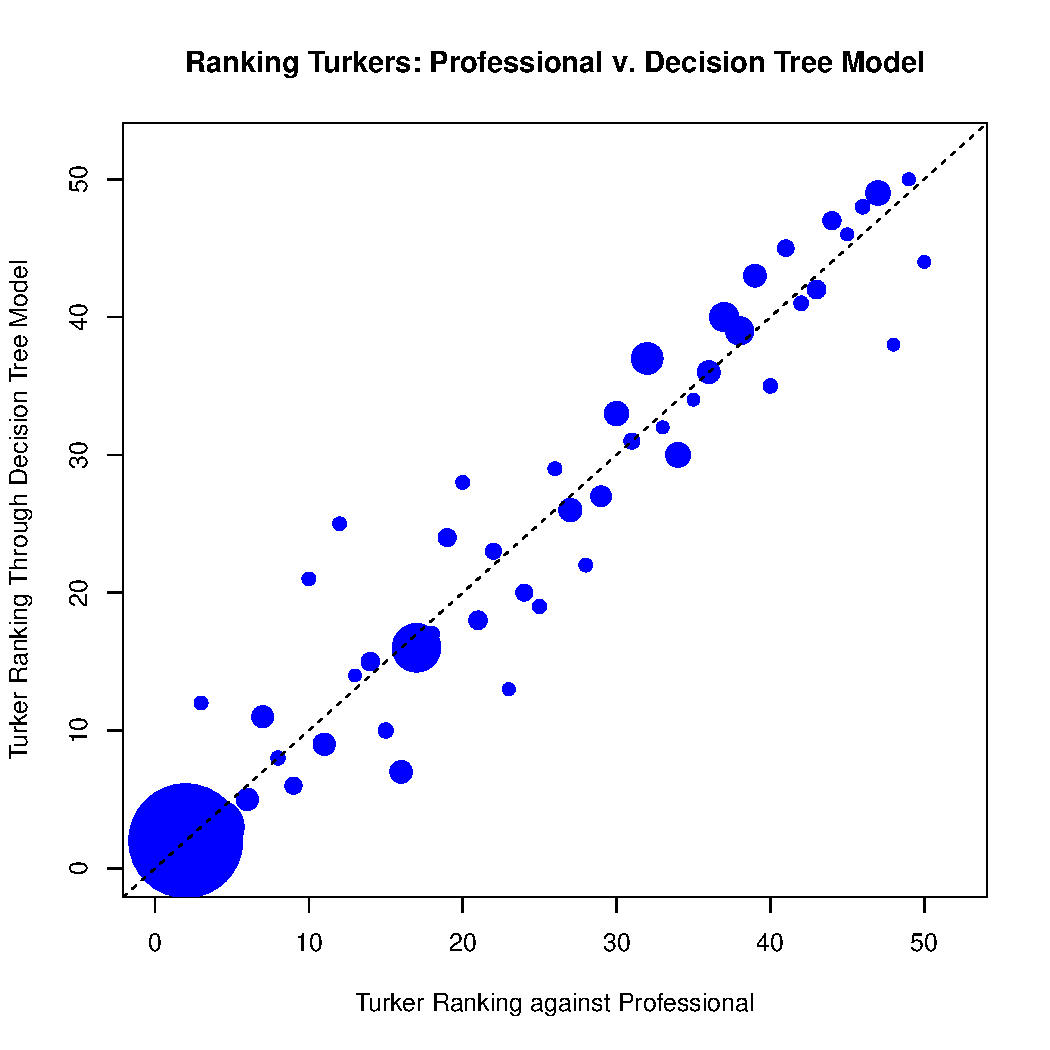
\includegraphics[width=\linewidth]{AllFeatureWithCali/allfeaturewithcaliorderdt.pdf}
  \caption{Relationship between gold standard raking and model predicted ranking. We use all features with calibration feature to train a Decision Tree model. }
    \label{fdtallcalirorder}
\end{figure}

\subsubsection{Linear Regression Model}
We train Linear Regression Model to rank workers.
\begin{table}[htbp]
\begin{center}
\begin{tabular}{| l | c | r |}
\hline \bf Feature Set & \bf Prson's  &\bf Sprman's  \\ \hline
Sentence features & na & na \\
Worker level feature & na  & na \\
Ranking feature & na & na \\
Calibration feature & na& na\\
All features (Calibration)& 0.97 & 0.97 \\
\hline
\end{tabular}
\end{center}
\caption{\label{tlrpearson} Pearson's Correlation for Linear Regression Model trained from different feature set }
\end{table}

We train Linear Regression Model using all features with calibration to rate workers and rank them.
Figure~\ref{flrallcalirorder} shows the relation between gold standard ranking and model predicted ranking.

\begin{figure}[htbp]
  \centering
  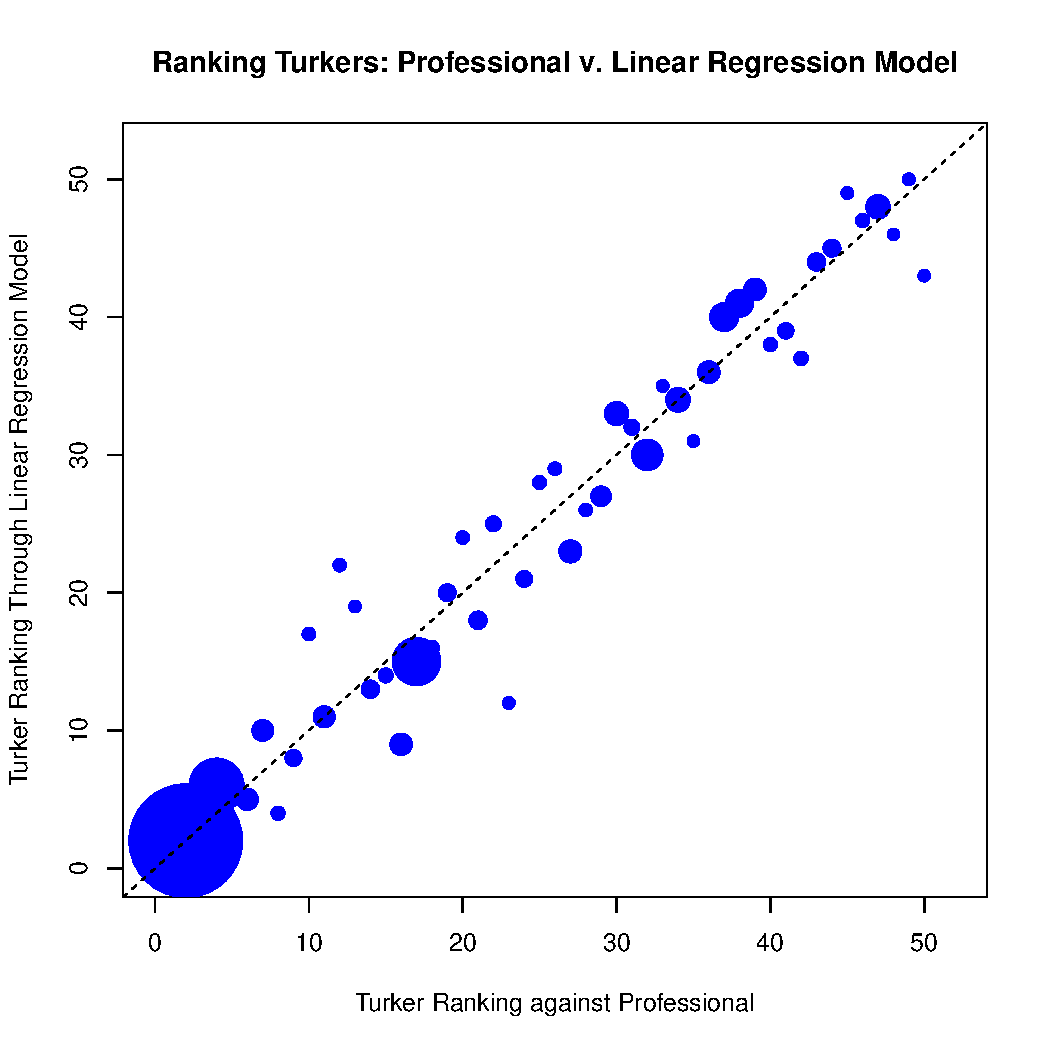
\includegraphics[width=\linewidth]{AllFeatureWithCali/allcalirankinglrorder.pdf}
  \caption{Relationship between gold standard raking and model predicted ranking. We use all features with calibration feature to train a Linear Regression model. }
    \label{flrallcalirorder}
\end{figure}
\subsubsection{Data Analysis} \label{dataanaly}

We analyze the data considering the timing information that accompanies the translations that we collected. In this analysis, we'd like to evaluate the performance of each worker as time goes on. Each worker translates one or more HITs. Since the translations were collected in two batches, which started at different times, we assign a relative time to each assignment to simulate what would have happened if both batches were run at the same time.  For each HIT, we assign it a relative time by calculating difference between the HIT's submission time and the HIT's creation time. This gives the HIT's relative submission time.  For each worker, we calculated the BLEU score for each of their HITs and analyze the translation quality of the worker at different time points. We are interested in seeing whether workers produce consistently good translations over time or if their quality drops off over time, and if workers who produce bad translations submit them more quickly than workers who submit good translations.  Figure~\ref{fworkerperf} illustrates workers' translation quality at across time. In this graph, each tick represent a single translation HIT, and depicts the HIT's BLEU score (color) and its size/number of sentences (thickness).  The worker who provided the translation is graphed on the y axis, and the submission time is plotted on the x axis. We set the median of all HITs' BLEU scores as the threshold. If the HIT's BLEU score is higher than the median, then the HIT's color is dark.  A light colored tick mark means the HIT's BLEU score is lower than the median. In Figure~\ref{fworkerperf}, the order of workers on y axis is based on the gold standard ranking of these workers. The top most worker ranked highest and the bottom most worker ranked lowest. 

From Figure~\ref{fworkerperf}, we see that most workers' performance stays
consistent as time passes. This is good, since it may enable us to predict workers' performance based on their early submission so that we can come to an early decision about whether to continue to hire them.  If we rank the worker based solely on their first HITs' BLEU score, comparing all sentences in that HIT against the reference translation, then we get a surprisingly strong correlation with the true gold standard ranking of workers based on all of their submitted work. The Spearman Correlation is 0.86 when comparing this first-HIT ranking with gold standard ranking.
\begin{figure}[htbp]
  \centering
  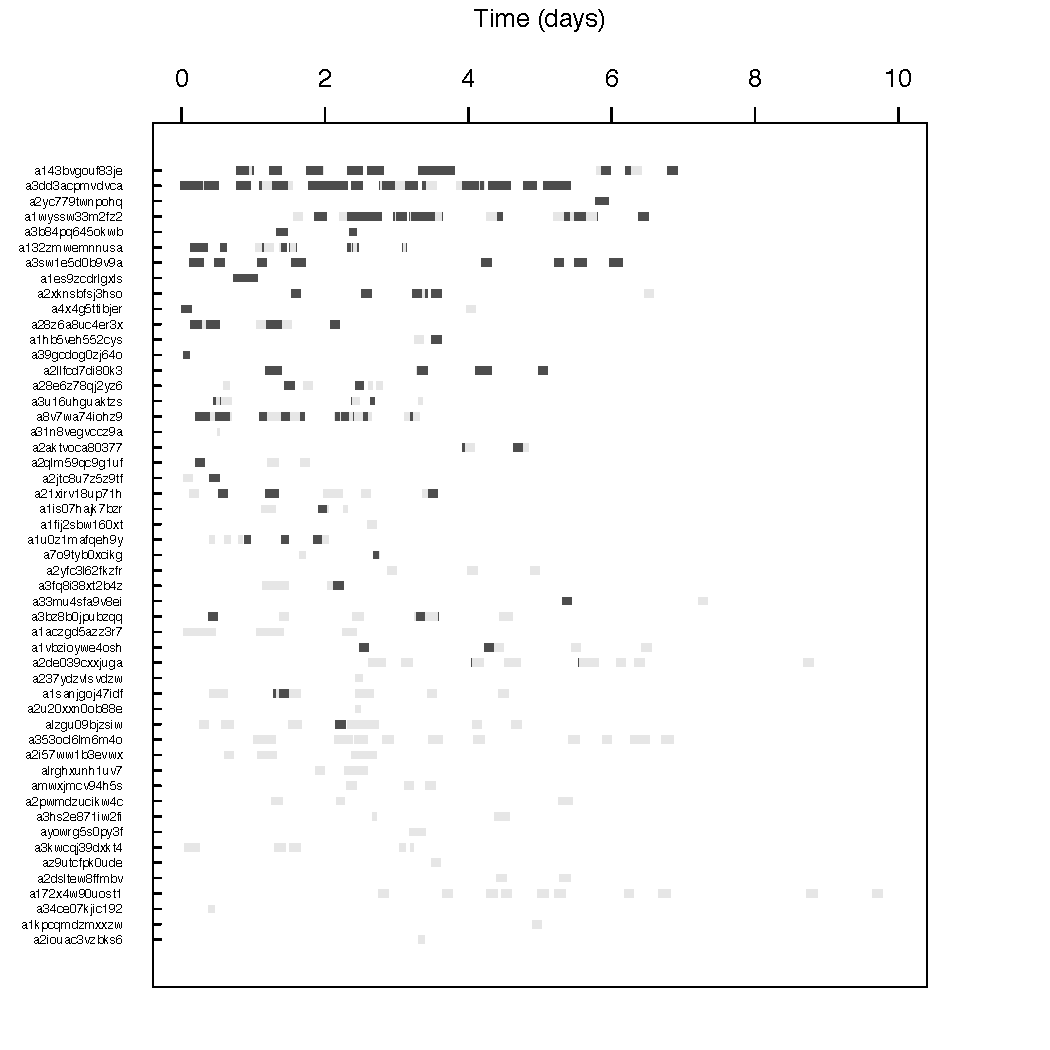
\includegraphics[width=\linewidth]{WorkerPerf/workerperform.pdf}
  \caption{Workers' performance  at across time.}
    \label{fworkerperf}
\end{figure}

Expanding the experiment mentioned above, we rank workers using their first $k$ HITs and calculate Spearman Correlation comparing against the gold standard ranking list (calculated over all HITs, instead of just the first $k$). The value of $k$ could range from 1 to the max number of HITs submitted by any single worker. Since some workers only translated a small number of HITs, larger values of $k$ will be greater than the total number of HITs that they provided. For those workers who translated less than $k$ HITs in total, we use all of the HITs they submitted to rate them.  Since the correlation converges to 1 after $k$ is larger than 10, we plot the graph to show the increase in correlation for $k$ from  1 to 10. Figure~\ref{fcorr} shows details.  The average number HITs each worker provided is 15.06, so we also plot Figure~\ref{fcorrnor} to show the percentage of HITs we use to rank workers for each value of $k$.

    

\begin{figure}[htbp]
  \centering
  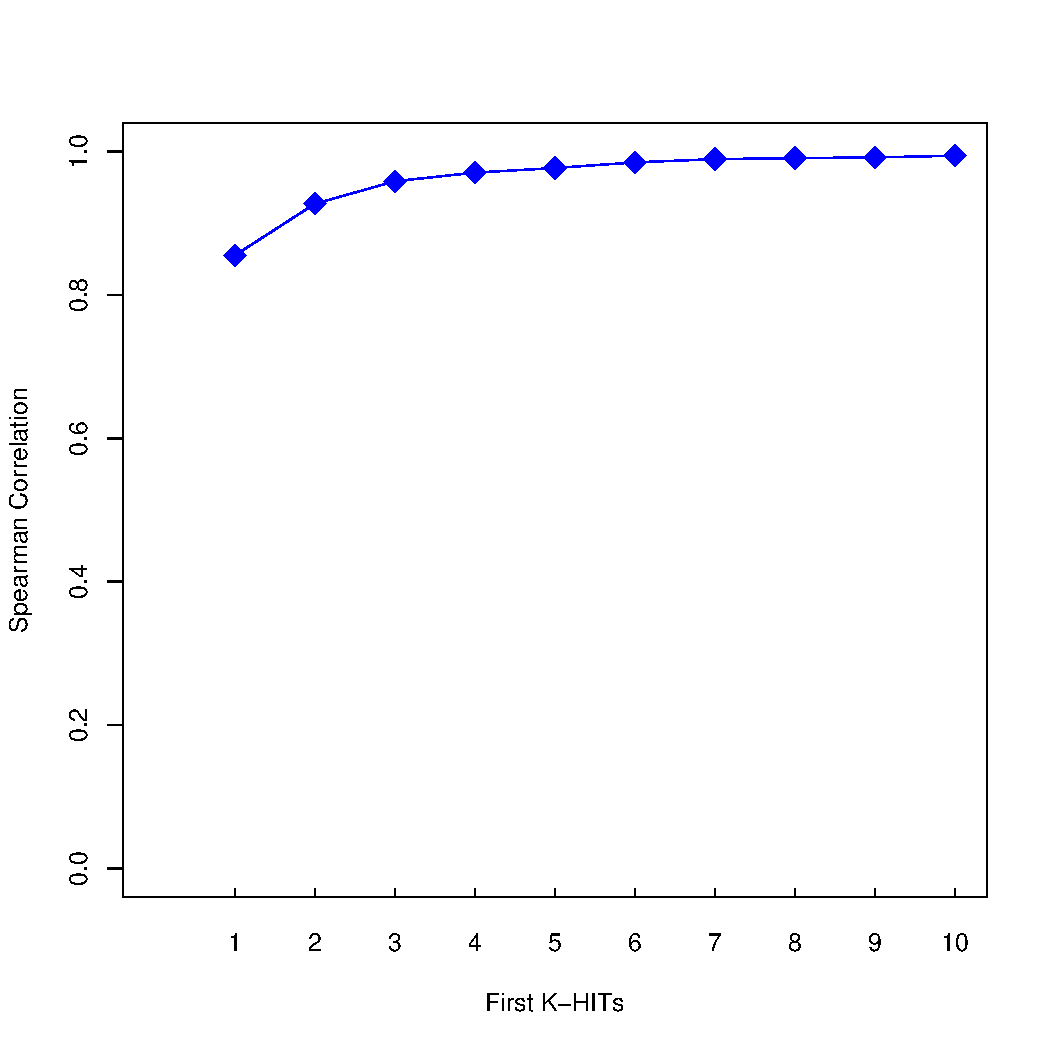
\includegraphics[width=\linewidth]{WorkerPerf/corr.pdf}
  \caption{Spearman Correlation with the gold standard as we rank the workers based on their first $k$ HITs}
    \label{fcorr}
\end{figure}

\begin{figure}[htbp]
  \centering
  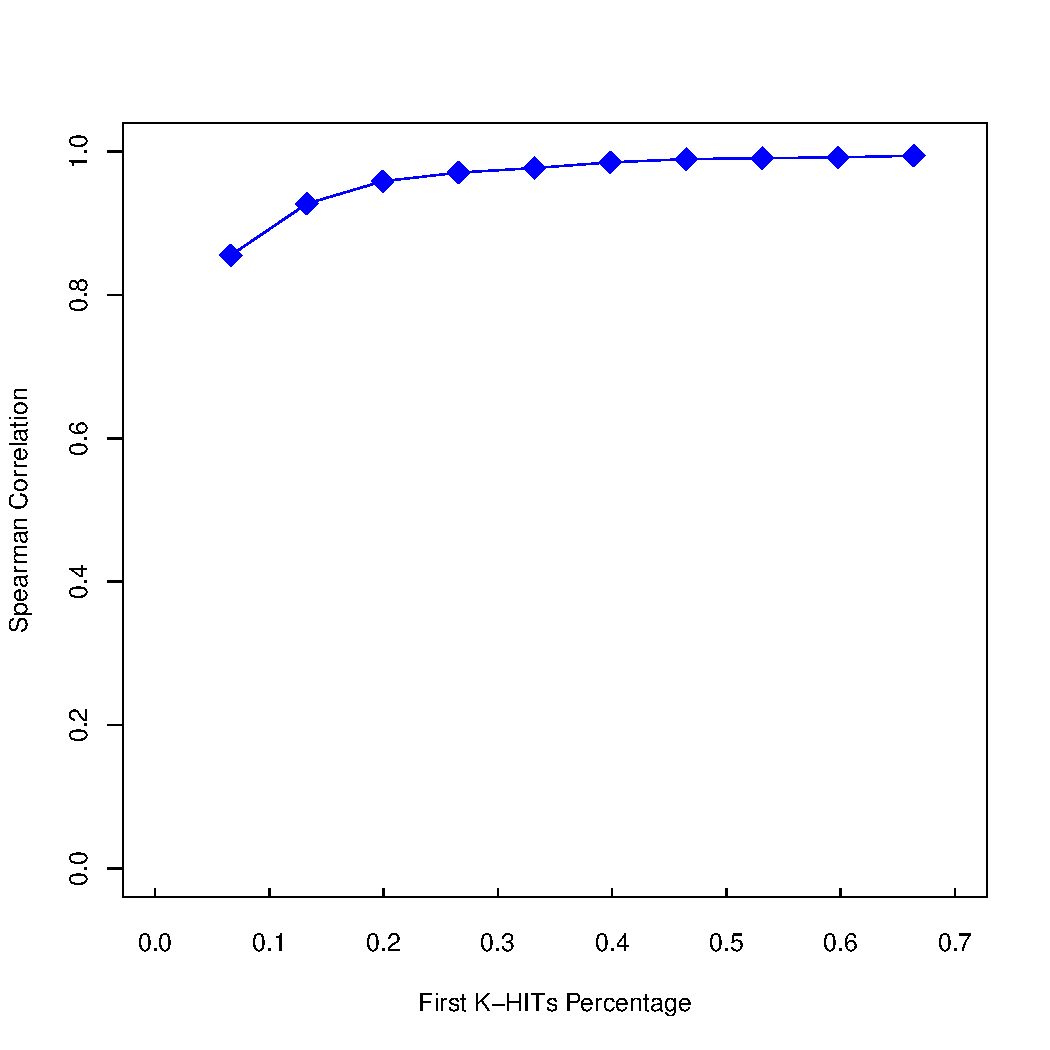
\includegraphics[width=\linewidth]{WorkerPerf/corrnormalized.pdf}
  \caption{The percentage of worker data used to rank them as $k$ increases}
    \label{fcorrnor}
\end{figure}
 \subsubsection{Cost Optimization}
There are two approaches that we use to reduce costs. In the first approach, we attempt to quickly rank workers and discard low ranking workers. In the second approach, we reduce the number of translations that we buy for each foreign sentence. After receiving a translation, we decide whether its quality is sufficient or whether we ought to pay for another translation (with the hope that the subsequent translation will be better).  In both cases we aim to reduce costs, while keeping our overall translation quality high.
 
 For the first approach, as mentioned in section~\ref{dataanaly}, we show we are able to rank workers accurately using only the translations of their first 4 HITs.  The ranked list of workers using 4 HITs is  almost identical to the gold standard ranking that uses all HITs. In other words, we can predict workers' performance reasonably well, as long as we have obtained a small number of HITs from them.  (Assuming that we have professional translations of their initial HITs, which we can use to calculate their translation quality). Consequently, we can decide whether to continue to hire a worker in a very short time after analyzing the first HIT(s) provided by each worker.
 
 For the second approach,  we train a model to decide whether a translation  is `good enough,' in which case we don't need to  pay for another redundant translation of the source sentence.  To perform this experiment, we divide the data into 3 parts: 10$\%$ of the data as a training set, 10$\%$ of the data as a validation set and the remaining 80$\%$ of the data as a test set. We train the model to score each translation we've got already, to use this score to evaluate whether to get another translation. The challenge is how to set the threshold to separate acceptable translations and unacceptable ones. 
 
 
% Maybe first describe the model features, and then describe how you set the threshold value. 
 In our design, we set the threshold empirically using the validation set after we have trained the model on the disjoint training set. More specifically, during the training process, we get the lower bound and upper bound of scores for translations in the training set. Then we search for the threshold through traversing from the lower bound to the upper bound by a small step size. %add a figure to illustrate the traversal
 We use each value  in the process  as the potential threshold.  We score translations of the foreign sentences in the validation set.  Since this approach assumes a temporal ordering of the translations, we compute the scores for each translation of a source sentence using the time-ordering of when Turkers submitted them. There are 2 conditions on the halt of this process for each foreign sentence: 1) the predicted BLEU score of some translation (submitted earlier than the last translation) is higher than the threshold or 2) we have scored all 4 translations.  

To evaluate the performance of the model running with different thresholds, we first compute an upper boud by selecting the best translation among all 4 candidates for each foreign sentence of the validation set according to our  model. We call this set $S_{upper}$.  $S_{upper}$ is the highest BLEU score we can get by choosing translation using the model, since it has access to all of the available translations.  

After we have used the validation set to sweep various threshold values,  we can pick a suitable value for the threshold by picking the lowest value that is within some delta of $S_{upper}$, say  90$\%$. 

Finally, we retrain our model using the union set of the training set and validation set, use the resulting model on the test set.  We evaluate the model's performance by counting the average number of candidate translations that it solicits per source sentence, and by computing the loss in overall BLEU score compared to when it had access to all 4 translations.  This evaluation shows how much money our model would save by eliminating unnecessary redundancy in the translation process, and how close it is to the upper bound on translation quality when using all of the translations from the original set.

\section{Related Work}
In the second approach mentioned above, we train models to separate acceptable and unacceptable translation candidates. Candidates with BLEU scores higher than the threshold are acceptable and vice versa. We search for the threshold on the validating set that is leading to the BLEU within some delta of $S_{upper}$.  The threshold between acceptable and unacceptable translations is fuzzy so there exists some uncertainty in labeling each data sample and we need to sweep various values. 

Repeated labeling \cite{sheng2008get} maybe one way to solve the problem of the  uncertainty in labeling and the fuzziness in the selection of the threshold. In the work of \cite{sheng2008get}, first they showed that for single-labeling examples, they showed that the labeling quality (the probability of correct labeling) is critical to the model quality. The model prediction accuracy rises as the labeling quality increases. However, in reality, we cannot always get high-quality labeled data samples with relatively low costs. To keep the model trained on noisy labeled data having a high accuracy in predicting , \newcite{sheng2008get} proposed repeated-labeling framework. 

In their work, \newcite{sheng2008get} assume each data sample's labeling is independent of the specific data point. Each repeated-labeling data sample is assigned an integrated label by majority voting. The experimental results show that repeated labeling can improve the model's predicting accuracy even if labels quality can not be guaranteed and are noisy.  As long as the integrated quality ( the probability of the integrated labeling being correct) is higher than 0.5, repeated labeling makes benefits for model training. More closer the quality to 0.5, the more benefits obtained in model prediction.

If we relax the condition on the uniform labeler quality and allow lablers to have different quality,  a new question arises: should we use the best individual labeler or should we combile the results from multiple labelers? According to the analysis,  it depends on how much the best labeler's quality is better the average quality of all labelers.

Majority voting is an useful approach to improve the quality of corpus. However, it omits  the uncertain property of data samples' labels and loses the information about uncertainty in labels. To take advantage of the uncertainty, \newcite{sheng2008get} represent labeling uncertainty in probability. For each unlabeled data sample $x_{i}$, the \textit{multiplied examples} (ME) procedure takes the existing multi-label set  $L_i = \{y_{ij}\}$ as input, and for each label value $y_{ij} $ in the multiset, make a replica of $x_i$ which is labeled $y_{ij}$, and use the probability of that label value appearing in the multi-label set as the weight of that replica . We can use cost-sensitive learning method to train model on the modified data set. Experiment shows that ME strategy is better than than majority voting.

In experiments, for each data set, 30\% data samples are held out as the test data, and the rest data is the "pool" from which we acquire unlabeled and labeled samples. When deciding the next data sample to be labeled, they use the generalized round robin strategy: selecting the data sample with the fewest labels. To make the selection more reasonable, they proposed the selective-repeated labeling method. For each data sample, $LU$ is defined as the label uncertainty which measures the labels' diversity on the data sample. Similarly, $MU$ is defined as the model uncertainty which measures the disagreement on models' prediction to the data sample. $LMU$ is defined as the label and model uncertainty which is the geometric average of $LU$ and $MU$. Instead of assigning the new label to  the data sample with fewest labels, they choose the data sample with the highest $LMU$ score and get benefits.

Outline of related work of 'Benefits of a Model of Annotation'.\\
1. Related Point: our work is trying to find the best translation from all candidates. Their work is trying to select a label from the multi-label set.
2. Different Point: our work is don't have labels but they have.

\newcite{passonneau2013benefits} created a Bayesian model of annotation, which they applied to the problem of word sense annotation. Rather than hiring professional annotators, which is very expensive, they hire non-expert annotators on Mechanical Turk.  They collected 20 to 25 word sense labels for each word. To decide which label to select for each word, and to compute the quality of the annotation and of the annotators, they proposed the probabilistic model. The prior probability  of each label is produced
\bibliographystyle{acl2012}
\bibliography{tacl.bib}

\end{document}